% 独自のコマンド

% ■ アブストラクト
%  \begin{jabstract} 〜 \end{jabstract}  :日本語のアブストラクト
%  \begin{eabstract} 〜 \end{eabstract}  :英語のアブストラクト

% ■ 謝辞
%  \begin{acknowledgment} 〜 \end{acknowledgment}

% ■ 文献リスト
%  \begin{bib}[100] 〜 \end{bib}


\newif\ifjapanese

\japanesetrue  % 論文全体を日本語で書く(英語で書くならコメントアウト)

\ifjapanese
  \documentclass[a4j,twoside,openright,11pt]{jreport} % 両面印刷の場合。余白を綴じ側に作って右起こし。
  %\documentclass[a4j,11pt]{jreport}                  % 片面印刷の場合。
  \renewcommand{\bibname}{参考文献}
  \newcommand{\acknowledgmentname}{謝辞}
\else
  \documentclass[a4paper,11pt]{report}
  \newcommand{\acknowledgmentname}{Acknowledgment}
\fi
\usepackage{thesis}
\usepackage{ascmac}
\usepackage{graphicx}
\usepackage{multirow}
\usepackage{url}
\bibliographystyle{jplain}

\bindermode  % バインダー用余白設定

% 日本語情報(必要なら)
\jclass  {修士論文}                             % 論文種別
\jtitle    {近接関係に基づく情報取得システム}    % タイトル。改行する場合は\\を入れる
\juniv    {慶應義塾大学大学院}                  % 大学名
\jfaculty  {政策・メディア研究科}               % 学部、学科
\jauthor  {郡山 隼人}                       % 著者
\jhyear  {26}                                   % 平成○年度
\jsyear  {2014}                                 % 西暦○年度
\jkeyword  {Bluetooth、近接、修士論文}     % 論文のキーワード
\jproject{インタラクションデザインプロジェクト} %プロジェクト名
\jdate{2015年1月}

% 英語情報(必要なら)
\eclass  {Master's Thesis}                            % 論文種別
\etitle    {Information gathering system based on proximity}      % タイトル。改行する場合は\\を入れる
\euniv  {Keio University}                             % 大学名
\efaculty  {Graduate School of Media and Governance}  % 学部、学科
\eauthor  {Hayato Koriyama}                           % 著者
\eyear  {2014}                                        % 西暦○年度
\ekeyword  {\LaTeX, Templete, Master Thesis}          % 論文のキーワード
\eproject{Interaction Design Project}                 %プロジェクト名
\edate{January 2015}





\begin{document}

\ifjapanese
  \jmaketitle    % 表紙(日本語)
\else
  \emaketitle    % 表紙(英語)
\fi

% ■ アブストラクトの出力 ■
%	◆書式:
%		begin{jabstract}〜end{jabstract}	:日本語のアブストラクト
%		begin{eabstract}〜end{eabstract}	:英語のアブストラクト
%		※ 不要ならばコマンドごと消せば出力されない。



% 日本語のアブストラクト
\begin{jabstract}

テンプレートの説明を、テンプレート自身を使って説明する。これは @kurokobo による卒業論文のための\LaTeX テンプレートを修士論文用に改造し、さらにUTF-8化やMakefile等の添付をしたものである。

この部分には一般には論文のアブストラクトを書く。日本語のアブストラクトを書きたいなら、\verb|\begin{jabstract}| と \verb|\end{jabstract}| の間に文章を書けば、今のこのページのように体裁が勝手に整って出力される。英語のアブストラクトは \verb|\begin{eabstract}| と \verb|\end{eabstract}| の間に書けば、次ページのような体裁で出力される。

両方を書けば、日本語と英語の両方のアブストラクトが並んで出力される(この文書はサンブルなので両方書いてある)。ページ順序は、コマンドを書いた順序の通り。どちらか一方のみを出力したい場合は、不要な方をコマンド自体を含め削除する。

このあたりの詳細もあとで書く。基本的には、{\tt main.tex}を上から順にいじっていけばできるはず。

\end{jabstract}



% 英語のアブストラクト
\begin{eabstract}

Eigo ga dekinai node Roma-ji de soreppoi hunniki wo daseruto iina.

Murippoi desu ne.

Write down your abstract here. Write down your abstract here. Write down your abstract here. Write down your abstract here. Write down your abstract here. Write down your abstract here.

 Write down your abstract here. Write down your abstract here. Write down your abstract here. Write down your abstract here. Write down your abstract here. Write down your abstract here. Write down your abstract here. Write down your abstract here. Write down your abstract here. Write down your abstract here. Write down your abstract here. Write down your abstract here.
 
Write down your abstract here. Write down your abstract here.

\end{eabstract}
  % アブストラクト。要独自コマンド、include先参照のこと

\tableofcontents  % 目次
\listoffigures    % 表目次
\listoftables    % 図目次

\pagenumbering{arabic}

\chapter{序論}
\label{chap:introduction}

論文は序論のようなもので始める。タイトルは序論でも序言でもはじめにでもいいけど、『序論』で始めたら『結論』で終わり、『序言』で始めたら『結言』で終わるようにする。『はじめに』なら『おわりに』で終わる。『序論』で始まって『おわりに』でおわるとか、そういうちぐはぐなのはだめ。

ここでは序論として書く。序論では、研究の背景やら目的やらを書くのが普通。今はテンプレートの説明なので、大して書くことは無い。


\section{背景}

ここではこのテンプレートのオリジナルの作者である @kurokobo の書いたもの\cite{kurokobo10}を引用したい。

\begin{quotation}
ぼくは別に\LaTeX に明るいわけではなくて、この研究室に所属してから初めて触った程度。四年生になってぼく自身が卒業論文を書くことになって、先生は\LaTeX を推奨していたんだけど、テンプレートありますかって聞いたら特にないから作ってほしいとのことだったので、じゃあ作りますよ、という流れ。ぼく自身が使いやすいように、自分が使いながらいろいろ改良をして、こうして公開している。

作成にあたっては、先輩方の卒業論文や主にぐーぐる先生を活用したインターネット上の情報を参考にした。

ただ、卒業論文の体裁は、それぞれの研究室の文化や、担当の指導教員のこだわりも強く影響することも事実。このテンプレートは、『ぼくが所属していた研究室』という、ごくごく限定的でローカルな仕様に沿ったフォーマット――より正確に言えば『ぼくが所属していた研究室ではNGではなかった』フォーマット――というだけのもの。そのあたり、承知の上で使ってほしい。

他の研究室で使う場合は、指導教員の許可を仰ぐほうが確実。
\end{quotation}

筆者はこの卒業論文用のテンプレートを大学院ガイドに例示されている体裁\cite{mag_guide12}に沿うように改造した。これは論文の形式で言えばもっと後ろに書いてあるべきことなのかもしれない。

\section{本文書の構成}

第1章の最後は、文書全体の構成を大まかに書くとよいらしい。

第\ref{chap:introduction}章では本テンプレートの概要みたいなものを書いた。第\ref{chap:howto}章では、本テンプレートの使い方を説明する。第\ref{chap:latex}章で図表や数式の挿入など代表的な\LaTeX コマンドを解説する。第\ref{chap:conclusion}章では、『序論』で始めたら『結論』で終われと書いた手前書かざるを得ないので、なにか結論らしいことを書く。付録として、テンプレートのサンプルになるように無理矢理ゴミを添付する。
  % 本文1
\chapter{本テンプレートの使い方}
\label{chap:howto}

本章では、本テンプレートの具体的な使用方法を解説する。基本的には、{\tt main.tex} を上から順に修正していけばよいだけ。 


\section{テンプレートの構成}

このテンプレートは、表\ref{tb:files}のファイルで構成されている。

\begin{table}[htbp]
  \caption{構成ファイル}
  \label{tb:files}
  \begin{center}\begin{tabular}{c|l}
    \hline
    ファイル名&用途\\\hline\hline
    {\tt main.tex}&メインのファイル。これを編集していく\\\hline
    {\tt thesis.sty}&論文のスタイルを定義したファイル。基本的には手は加えない\\\hline
    {\tt *.tex}&{\tt main.tex}に{\tt include}されるファイル群\\\hline
    {\tt *.eps}&画像ファイル\\\hline
    {\tt main.bib}&参考文献用のBibTeXファイル\\\hline
    {\tt Makefile}&Makefile。次節以降で説明\\\hline
    {\tt .gitignore}&Git用設定ファイル\\\hline
  \end{tabular}\end{center}
\end{table}

\section{コンパイル}
このテンプレートの\LaTeX ファイルをコンパイルしてPDFファイルを生成するには、ターミナルを開いて以下のようにする。

\begin{itembox}[l]{コマンド実行例}
\begin{verbatim}
% make
\end{verbatim}
\end{itembox}

こうすることで、\verb|platex|コマンド、\verb|pbibtex|コマンド、\verb|platex|コマンド2回、\verb|dvipdfmx|コマンドが全て実行され、{\tt main.pdf}が生成される。

コンパイルによって生成されたファイルを全て消すには、以下のようにする。

\begin{itembox}[l]{コマンド実行例}
\begin{verbatim}
% make clean
\end{verbatim}
\end{itembox}

\section{設定}

以下、{\tt main.tex}に対して行うべき設定を、このファイルの中に書いてある順に沿って説明する。

\subsection{論文全体の言語の設定}
\label{sec:lang}

\begin{itembox}[l]{{\tt main.tex}}
\begin{verbatim}
\japanesetrue	% 論文全体を日本語で書く(英語で書くならコメントアウト)
\end{verbatim}
\end{itembox}

ここでは論文全体の言語を設定する。日本語に設定すれば、『章』『目次』『謝辞』などが日本語で出力されて、行頭のインデントなども日本語の仕様になる。英語にした場合は、これらはそれぞれ『Chapter』『Table of Contents』『Acknowledgment』な体裁になる。インデントも行間も、英語用の設定が適用される。

\verb|\japanesetrue| をコメントアウトしなければ日本語に、コメントアウトすれば英語に設定される。


\subsection{余白の設定}

\begin{itembox}[l]{{\tt main.tex}}
\begin{verbatim}
\bindermode	% バインダ用余白設定
\end{verbatim}
\end{itembox}

このテンプレートの出力はA4用紙。ここではこれの四辺の余白を設定する。

最終的にバインダーで綴じて提出する場合、余白を左右対称にしてしまうと、見かけ上のバランスがとても悪くなる。これを解消するため、あらかじめ左側の余白を大きく取っておく。

\verb|\bindermode| をコメントアウトしなければ左綴じ用の余白に、コメントアウトすれば左右対称の余白に設定される。

両面印刷の場合、偶数ページと奇数ページで余白を広くとるべき側が違うので、\verb|documentclass| でこれを設定する。

\begin{itembox}[l]{{\tt main.tex}}
\begin{verbatim}
% 両面印刷の場合。余白を綴じ側に作って右起こし。
\documentclass[a4j,twoside,openright,11pt]{jreport}
% 片面印刷の場合。
%\documentclass[a4j,11pt]{jreport}
\end{verbatim}
\end{itembox}

両面印刷の場合は \verb|twoside| を使用する。\verb|openright| を使うと章のはじまりが必ず右側のページに来るようになる。

\subsection{論文情報の設定}
\label{sec:meta}

\begin{itembox}[l]{{\tt main.tex}}
\begin{verbatim}
% 日本語情報(必要なら)
\jclass  {修士論文}                             % 論文種別
\jtitle    {修士論文用 \LaTeX\ テンプレート}    % タイトル。改行する場合は\\を入れる
\juniv    {慶應義塾大学大学院}                  % 大学名
\jfaculty  {政策・メディア研究科}               % 学部、学科
\jauthor  {ほげ山 ふう助}                       % 著者
\jhyear  {24}                                   % 平成○年度
\jsyear  {2012}                                 % 西暦○年度
\jkeyword  {\LaTeX、テンプレート、修士論文}     % 論文のキーワード
\jproject{インタラクションデザインプロジェクト} %プロジェクト名
\jdate{2013年1月}

% 英語情報(必要なら)
\eclass  {Master's Thesis}                            % 論文種別
\etitle    {A \LaTeX Template for Master Thesis}      % タイトル。改行する場合は\\を入れる
\euniv  {Keio University}                             % 大学名
\efaculty  {Graduate School of Media and Governance}  % 学部、学科
\eauthor  {Fusuke Hogeyama}                           % 著者
\eyear  {2012}                                        % 西暦○年度
\ekeyword  {\LaTeX, Templete, Master Thesis}          % 論文のキーワード
\eproject{Interaction Design Project}                 %プロジェクト名
\edate{January 2013}
\end{verbatim}
\end{itembox}

ここでは論文のタイトルや著者の氏名などのメタデータを記述する。ここで書いたデータは、表紙とアブストラクトのページに使われる。必ずしも日本語と英語の両方を設定しなければいけないわけではなくて、自分が必要とする方だけ記述すればよい。

タイトルが長過ぎる場合は、表紙やアブストラクトのページでは自動で折り返して出力される。もし改行位置を自分で指定したい場合は、その場所に \verb|\\| を入力する。


\section{出力}

\verb|\begin{document}| から \verb|\end{document}| に記述した部分が、実際に{\tt DVI}(最終的には{\tt PDF})ファイルとして出力される。

\subsection{外部ファイルの読み込み({\tt include})}

出力部分の具体的な説明の前に、外部ファイルを読み込む方法を説明する。

\verb|\begin{document}| から \verb|\end{document}| の間では、\verb|\include| コマンドを使うことで、別の {\tt *.tex} ファイルを読み込ませられる。 

\begin{itembox}[l]{{\tt include}しない場合}
\begin{itembox}[l]{{\tt main.tex}}
\begin{verbatim}
\begin{document}
  \begin{jabstract}
  ほげほげ
  \end{jabstract}
\end{document}
\end{verbatim}
\end{itembox}
\end{itembox}

\begin{itembox}[l]{{\tt include}する場合}
\begin{minipage}{0.5\hsize}
\begin{itembox}[l]{{\tt main.tex}}
\begin{verbatim}
\begin{document}
\chapter{序論}
\label{chap:introduction}

論文は序論のようなもので始める。タイトルは序論でも序言でもはじめにでもいいけど、『序論』で始めたら『結論』で終わり、『序言』で始めたら『結言』で終わるようにする。『はじめに』なら『おわりに』で終わる。『序論』で始まって『おわりに』でおわるとか、そういうちぐはぐなのはだめ。

ここでは序論として書く。序論では、研究の背景やら目的やらを書くのが普通。今はテンプレートの説明なので、大して書くことは無い。


\section{背景}

ここではこのテンプレートのオリジナルの作者である @kurokobo の書いたもの\cite{kurokobo10}を引用したい。

\begin{quotation}
ぼくは別に\LaTeX に明るいわけではなくて、この研究室に所属してから初めて触った程度。四年生になってぼく自身が卒業論文を書くことになって、先生は\LaTeX を推奨していたんだけど、テンプレートありますかって聞いたら特にないから作ってほしいとのことだったので、じゃあ作りますよ、という流れ。ぼく自身が使いやすいように、自分が使いながらいろいろ改良をして、こうして公開している。

作成にあたっては、先輩方の卒業論文や主にぐーぐる先生を活用したインターネット上の情報を参考にした。

ただ、卒業論文の体裁は、それぞれの研究室の文化や、担当の指導教員のこだわりも強く影響することも事実。このテンプレートは、『ぼくが所属していた研究室』という、ごくごく限定的でローカルな仕様に沿ったフォーマット――より正確に言えば『ぼくが所属していた研究室ではNGではなかった』フォーマット――というだけのもの。そのあたり、承知の上で使ってほしい。

他の研究室で使う場合は、指導教員の許可を仰ぐほうが確実。
\end{quotation}

筆者はこの卒業論文用のテンプレートを大学院ガイドに例示されている体裁\cite{mag_guide12}に沿うように改造した。これは論文の形式で言えばもっと後ろに書いてあるべきことなのかもしれない。

\section{本文書の構成}

第1章の最後は、文書全体の構成を大まかに書くとよいらしい。

第\ref{chap:introduction}章では本テンプレートの概要みたいなものを書いた。第\ref{chap:howto}章では、本テンプレートの使い方を説明する。第\ref{chap:latex}章で図表や数式の挿入など代表的な\LaTeX コマンドを解説する。第\ref{chap:conclusion}章では、『序論』で始めたら『結論』で終われと書いた手前書かざるを得ないので、なにか結論らしいことを書く。付録として、テンプレートのサンプルになるように無理矢理ゴミを添付する。
 % 01.texをinclude
\end{document}
\end{verbatim}
\end{itembox}
\end{minipage}
\begin{minipage}{0.5\hsize}
\begin{itembox}[l]{{\tt 01.tex}}
\begin{verbatim}
\begin{jabstract}
ほげほげ
\end{jabstract}
\end{verbatim}
\end{itembox}
\end{minipage}
\end{itembox}

{\tt include}しない場合とする場合を比較するとこのとおり。どちらも出力結果は一緒。{\tt include}する場合は、読み込ませたい箇所に、読み込ませたい{\tt *.tex}ファイルの名前を、拡張子を除いて \verb|\include| コマンドで書けばよい。

\verb|\include| コマンドを用いるか用いないかは、たぶん文書量や個人の好みに依る。例えば章ごとに別のファイルにしておけば、修正箇所を探すときの手間が多少は省けるかもしれない。Gitで人と共有しつつ校正を頼むときにもファイルが分かれていたほうがコンフリクトを起こしにくい。


\subsection{表紙の出力}

\begin{itembox}[l]{{\tt main.tex}}
\begin{verbatim}
\ifjapanese
  \jmaketitle    % 表紙(日本語)
\else
  \emaketitle    % 表紙(英語)
\fi
\end{verbatim}
\end{itembox}

最初に、表紙を出力する。

\verb|\jmaketitle| が実行されると日本語の表紙が、\verb|\emaketitle| が実行されると英語の表紙がそれぞれ出力される。日本語の表紙には、第\ref{sec:meta}節で設定したうちの日本語の情報が、英語の表紙には同節で設定したうち英語の情報が、それぞれ参照されて、表記される。

デフォルトでは第\ref{sec:lang}説で設定した言語の表紙のみが出力されるようになっている。

\subsection{アブストラクトの出力}

\begin{itembox}[l]{{\tt main.tex}}
\begin{verbatim}
% ■ アブストラクトの出力 ■
%	◆書式:
%		begin{jabstract}〜end{jabstract}	:日本語のアブストラクト
%		begin{eabstract}〜end{eabstract}	:英語のアブストラクト
%		※ 不要ならばコマンドごと消せば出力されない。



% 日本語のアブストラクト
\begin{jabstract}

テンプレートの説明を、テンプレート自身を使って説明する。これは @kurokobo による卒業論文のための\LaTeX テンプレートを修士論文用に改造し、さらにUTF-8化やMakefile等の添付をしたものである。

この部分には一般には論文のアブストラクトを書く。日本語のアブストラクトを書きたいなら、\verb|\begin{jabstract}| と \verb|\end{jabstract}| の間に文章を書けば、今のこのページのように体裁が勝手に整って出力される。英語のアブストラクトは \verb|\begin{eabstract}| と \verb|\end{eabstract}| の間に書けば、次ページのような体裁で出力される。

両方を書けば、日本語と英語の両方のアブストラクトが並んで出力される(この文書はサンブルなので両方書いてある)。ページ順序は、コマンドを書いた順序の通り。どちらか一方のみを出力したい場合は、不要な方をコマンド自体を含め削除する。

このあたりの詳細もあとで書く。基本的には、{\tt main.tex}を上から順にいじっていけばできるはず。

\end{jabstract}



% 英語のアブストラクト
\begin{eabstract}

Eigo ga dekinai node Roma-ji de soreppoi hunniki wo daseruto iina.

Murippoi desu ne.

Write down your abstract here. Write down your abstract here. Write down your abstract here. Write down your abstract here. Write down your abstract here. Write down your abstract here.

 Write down your abstract here. Write down your abstract here. Write down your abstract here. Write down your abstract here. Write down your abstract here. Write down your abstract here. Write down your abstract here. Write down your abstract here. Write down your abstract here. Write down your abstract here. Write down your abstract here. Write down your abstract here.
 
Write down your abstract here. Write down your abstract here.

\end{eabstract}
	% アブストラクト。要独自コマンド、include先参照のこと
\end{verbatim}
\end{itembox}

表紙の次は、アブストラクト。

アブストラクトを出力するには、出力したい位置に、指定のコマンドを用いて文章を書き下せばよい。{\tt main.tex}に直接書いてもよいし、先述した \verb|\include| コマンドを利用して{\tt include}してもよい。

\verb|\begin{jabstract}| から \verb|\end{jabstract}| の間に書いた文章が日本語のアブストラクトとして、\verb|\begin{eabstract}| から \verb|\end{eabstract}| の間に書いた文章が英語のアブストラクトとして、それぞれ独立したページに出力される。

アブストラクトのページには、論文のタイトルやキーワードなどが、第\ref{sec:meta}節で設定した情報をもとにして自動で表記される。

日本語か英語のどちらか一方のみでよい場合は、不要な言語の方のコマンドを削除すればよい。これは、\verb|\begin| と \verb|\end| というコマンド自身も含めて削除する、ということで、\verb|\begin| と \verb|\end| の間を空っぽにするという意味ではないので注意。



\subsection{目次類の出力}
\label{sec:toc}

\begin{itembox}[l]{{\tt main.tex}}
\begin{verbatim}
\tableofcontents	% 目次
\listoffigures		% 表目次
\listoftables		% 図目次
\end{verbatim}
\end{itembox}

アブストラクトの次に、目次。文書の目次、図の目次、表の目次の三種類。

目次類を出力するには、出力したい位置に指定のコマンドを書けばよい。

これらのコマンドは、コンパイル時点での一時ファイル\footnote{{\tt *.toc}、{\tt *.lof}、{\tt *.lot}}の情報を、目次として体裁を整えて出力するもの。一時ファイルは、\verb|\begin{document}| から \verb|\end{document}| の間の章や節、図や表をコンパイルするときに、ついでに情報を取得しておいて生成される。

つまり気をつけなければいけないのは、コンパイルを一回しただけでは、一時ファイルが最新の状態に更新されるだけで、肝心の目次は正しい情報では出力されないということ。目次類を正しい情報で出力するには、最低二回のコンパイルが必要。一回目のコンパイルで一時ファイルが最新の情報に更新されて、二回目のコンパイルで初めて、その最新の一時ファイルの情報をもとに目次が出力される。

だから、文書に何らかの修正をして保存したあとは、最低でも二回、連続してコンパイルしないといけないことに注意する。

図や表を一つも使用していない場合は、目次名のみが書かれた空白のページが出力される。もしこれが不要な場合は、該当するコマンドをコメントアウトすればよい。


\subsection{本文の出力}

\begin{itembox}[l]{{\tt main.tex}}
\begin{verbatim}
\chapter{序論}
\label{chap:introduction}

論文は序論のようなもので始める。タイトルは序論でも序言でもはじめにでもいいけど、『序論』で始めたら『結論』で終わり、『序言』で始めたら『結言』で終わるようにする。『はじめに』なら『おわりに』で終わる。『序論』で始まって『おわりに』でおわるとか、そういうちぐはぐなのはだめ。

ここでは序論として書く。序論では、研究の背景やら目的やらを書くのが普通。今はテンプレートの説明なので、大して書くことは無い。


\section{背景}

ここではこのテンプレートのオリジナルの作者である @kurokobo の書いたもの\cite{kurokobo10}を引用したい。

\begin{quotation}
ぼくは別に\LaTeX に明るいわけではなくて、この研究室に所属してから初めて触った程度。四年生になってぼく自身が卒業論文を書くことになって、先生は\LaTeX を推奨していたんだけど、テンプレートありますかって聞いたら特にないから作ってほしいとのことだったので、じゃあ作りますよ、という流れ。ぼく自身が使いやすいように、自分が使いながらいろいろ改良をして、こうして公開している。

作成にあたっては、先輩方の卒業論文や主にぐーぐる先生を活用したインターネット上の情報を参考にした。

ただ、卒業論文の体裁は、それぞれの研究室の文化や、担当の指導教員のこだわりも強く影響することも事実。このテンプレートは、『ぼくが所属していた研究室』という、ごくごく限定的でローカルな仕様に沿ったフォーマット――より正確に言えば『ぼくが所属していた研究室ではNGではなかった』フォーマット――というだけのもの。そのあたり、承知の上で使ってほしい。

他の研究室で使う場合は、指導教員の許可を仰ぐほうが確実。
\end{quotation}

筆者はこの卒業論文用のテンプレートを大学院ガイドに例示されている体裁\cite{mag_guide12}に沿うように改造した。これは論文の形式で言えばもっと後ろに書いてあるべきことなのかもしれない。

\section{本文書の構成}

第1章の最後は、文書全体の構成を大まかに書くとよいらしい。

第\ref{chap:introduction}章では本テンプレートの概要みたいなものを書いた。第\ref{chap:howto}章では、本テンプレートの使い方を説明する。第\ref{chap:latex}章で図表や数式の挿入など代表的な\LaTeX コマンドを解説する。第\ref{chap:conclusion}章では、『序論』で始めたら『結論』で終われと書いた手前書かざるを得ないので、なにか結論らしいことを書く。付録として、テンプレートのサンプルになるように無理矢理ゴミを添付する。
	% 本文1
\chapter{本テンプレートの使い方}
\label{chap:howto}

本章では、本テンプレートの具体的な使用方法を解説する。基本的には、{\tt main.tex} を上から順に修正していけばよいだけ。 


\section{テンプレートの構成}

このテンプレートは、表\ref{tb:files}のファイルで構成されている。

\begin{table}[htbp]
  \caption{構成ファイル}
  \label{tb:files}
  \begin{center}\begin{tabular}{c|l}
    \hline
    ファイル名&用途\\\hline\hline
    {\tt main.tex}&メインのファイル。これを編集していく\\\hline
    {\tt thesis.sty}&論文のスタイルを定義したファイル。基本的には手は加えない\\\hline
    {\tt *.tex}&{\tt main.tex}に{\tt include}されるファイル群\\\hline
    {\tt *.eps}&画像ファイル\\\hline
    {\tt main.bib}&参考文献用のBibTeXファイル\\\hline
    {\tt Makefile}&Makefile。次節以降で説明\\\hline
    {\tt .gitignore}&Git用設定ファイル\\\hline
  \end{tabular}\end{center}
\end{table}

\section{コンパイル}
このテンプレートの\LaTeX ファイルをコンパイルしてPDFファイルを生成するには、ターミナルを開いて以下のようにする。

\begin{itembox}[l]{コマンド実行例}
\begin{verbatim}
% make
\end{verbatim}
\end{itembox}

こうすることで、\verb|platex|コマンド、\verb|pbibtex|コマンド、\verb|platex|コマンド2回、\verb|dvipdfmx|コマンドが全て実行され、{\tt main.pdf}が生成される。

コンパイルによって生成されたファイルを全て消すには、以下のようにする。

\begin{itembox}[l]{コマンド実行例}
\begin{verbatim}
% make clean
\end{verbatim}
\end{itembox}

\section{設定}

以下、{\tt main.tex}に対して行うべき設定を、このファイルの中に書いてある順に沿って説明する。

\subsection{論文全体の言語の設定}
\label{sec:lang}

\begin{itembox}[l]{{\tt main.tex}}
\begin{verbatim}
\japanesetrue	% 論文全体を日本語で書く(英語で書くならコメントアウト)
\end{verbatim}
\end{itembox}

ここでは論文全体の言語を設定する。日本語に設定すれば、『章』『目次』『謝辞』などが日本語で出力されて、行頭のインデントなども日本語の仕様になる。英語にした場合は、これらはそれぞれ『Chapter』『Table of Contents』『Acknowledgment』な体裁になる。インデントも行間も、英語用の設定が適用される。

\verb|\japanesetrue| をコメントアウトしなければ日本語に、コメントアウトすれば英語に設定される。


\subsection{余白の設定}

\begin{itembox}[l]{{\tt main.tex}}
\begin{verbatim}
\bindermode	% バインダ用余白設定
\end{verbatim}
\end{itembox}

このテンプレートの出力はA4用紙。ここではこれの四辺の余白を設定する。

最終的にバインダーで綴じて提出する場合、余白を左右対称にしてしまうと、見かけ上のバランスがとても悪くなる。これを解消するため、あらかじめ左側の余白を大きく取っておく。

\verb|\bindermode| をコメントアウトしなければ左綴じ用の余白に、コメントアウトすれば左右対称の余白に設定される。

両面印刷の場合、偶数ページと奇数ページで余白を広くとるべき側が違うので、\verb|documentclass| でこれを設定する。

\begin{itembox}[l]{{\tt main.tex}}
\begin{verbatim}
% 両面印刷の場合。余白を綴じ側に作って右起こし。
\documentclass[a4j,twoside,openright,11pt]{jreport}
% 片面印刷の場合。
%\documentclass[a4j,11pt]{jreport}
\end{verbatim}
\end{itembox}

両面印刷の場合は \verb|twoside| を使用する。\verb|openright| を使うと章のはじまりが必ず右側のページに来るようになる。

\subsection{論文情報の設定}
\label{sec:meta}

\begin{itembox}[l]{{\tt main.tex}}
\begin{verbatim}
% 日本語情報(必要なら)
\jclass  {修士論文}                             % 論文種別
\jtitle    {修士論文用 \LaTeX\ テンプレート}    % タイトル。改行する場合は\\を入れる
\juniv    {慶應義塾大学大学院}                  % 大学名
\jfaculty  {政策・メディア研究科}               % 学部、学科
\jauthor  {ほげ山 ふう助}                       % 著者
\jhyear  {24}                                   % 平成○年度
\jsyear  {2012}                                 % 西暦○年度
\jkeyword  {\LaTeX、テンプレート、修士論文}     % 論文のキーワード
\jproject{インタラクションデザインプロジェクト} %プロジェクト名
\jdate{2013年1月}

% 英語情報(必要なら)
\eclass  {Master's Thesis}                            % 論文種別
\etitle    {A \LaTeX Template for Master Thesis}      % タイトル。改行する場合は\\を入れる
\euniv  {Keio University}                             % 大学名
\efaculty  {Graduate School of Media and Governance}  % 学部、学科
\eauthor  {Fusuke Hogeyama}                           % 著者
\eyear  {2012}                                        % 西暦○年度
\ekeyword  {\LaTeX, Templete, Master Thesis}          % 論文のキーワード
\eproject{Interaction Design Project}                 %プロジェクト名
\edate{January 2013}
\end{verbatim}
\end{itembox}

ここでは論文のタイトルや著者の氏名などのメタデータを記述する。ここで書いたデータは、表紙とアブストラクトのページに使われる。必ずしも日本語と英語の両方を設定しなければいけないわけではなくて、自分が必要とする方だけ記述すればよい。

タイトルが長過ぎる場合は、表紙やアブストラクトのページでは自動で折り返して出力される。もし改行位置を自分で指定したい場合は、その場所に \verb|\\| を入力する。


\section{出力}

\verb|\begin{document}| から \verb|\end{document}| に記述した部分が、実際に{\tt DVI}(最終的には{\tt PDF})ファイルとして出力される。

\subsection{外部ファイルの読み込み({\tt include})}

出力部分の具体的な説明の前に、外部ファイルを読み込む方法を説明する。

\verb|\begin{document}| から \verb|\end{document}| の間では、\verb|\include| コマンドを使うことで、別の {\tt *.tex} ファイルを読み込ませられる。 

\begin{itembox}[l]{{\tt include}しない場合}
\begin{itembox}[l]{{\tt main.tex}}
\begin{verbatim}
\begin{document}
  \begin{jabstract}
  ほげほげ
  \end{jabstract}
\end{document}
\end{verbatim}
\end{itembox}
\end{itembox}

\begin{itembox}[l]{{\tt include}する場合}
\begin{minipage}{0.5\hsize}
\begin{itembox}[l]{{\tt main.tex}}
\begin{verbatim}
\begin{document}
\chapter{序論}
\label{chap:introduction}

論文は序論のようなもので始める。タイトルは序論でも序言でもはじめにでもいいけど、『序論』で始めたら『結論』で終わり、『序言』で始めたら『結言』で終わるようにする。『はじめに』なら『おわりに』で終わる。『序論』で始まって『おわりに』でおわるとか、そういうちぐはぐなのはだめ。

ここでは序論として書く。序論では、研究の背景やら目的やらを書くのが普通。今はテンプレートの説明なので、大して書くことは無い。


\section{背景}

ここではこのテンプレートのオリジナルの作者である @kurokobo の書いたもの\cite{kurokobo10}を引用したい。

\begin{quotation}
ぼくは別に\LaTeX に明るいわけではなくて、この研究室に所属してから初めて触った程度。四年生になってぼく自身が卒業論文を書くことになって、先生は\LaTeX を推奨していたんだけど、テンプレートありますかって聞いたら特にないから作ってほしいとのことだったので、じゃあ作りますよ、という流れ。ぼく自身が使いやすいように、自分が使いながらいろいろ改良をして、こうして公開している。

作成にあたっては、先輩方の卒業論文や主にぐーぐる先生を活用したインターネット上の情報を参考にした。

ただ、卒業論文の体裁は、それぞれの研究室の文化や、担当の指導教員のこだわりも強く影響することも事実。このテンプレートは、『ぼくが所属していた研究室』という、ごくごく限定的でローカルな仕様に沿ったフォーマット――より正確に言えば『ぼくが所属していた研究室ではNGではなかった』フォーマット――というだけのもの。そのあたり、承知の上で使ってほしい。

他の研究室で使う場合は、指導教員の許可を仰ぐほうが確実。
\end{quotation}

筆者はこの卒業論文用のテンプレートを大学院ガイドに例示されている体裁\cite{mag_guide12}に沿うように改造した。これは論文の形式で言えばもっと後ろに書いてあるべきことなのかもしれない。

\section{本文書の構成}

第1章の最後は、文書全体の構成を大まかに書くとよいらしい。

第\ref{chap:introduction}章では本テンプレートの概要みたいなものを書いた。第\ref{chap:howto}章では、本テンプレートの使い方を説明する。第\ref{chap:latex}章で図表や数式の挿入など代表的な\LaTeX コマンドを解説する。第\ref{chap:conclusion}章では、『序論』で始めたら『結論』で終われと書いた手前書かざるを得ないので、なにか結論らしいことを書く。付録として、テンプレートのサンプルになるように無理矢理ゴミを添付する。
 % 01.texをinclude
\end{document}
\end{verbatim}
\end{itembox}
\end{minipage}
\begin{minipage}{0.5\hsize}
\begin{itembox}[l]{{\tt 01.tex}}
\begin{verbatim}
\begin{jabstract}
ほげほげ
\end{jabstract}
\end{verbatim}
\end{itembox}
\end{minipage}
\end{itembox}

{\tt include}しない場合とする場合を比較するとこのとおり。どちらも出力結果は一緒。{\tt include}する場合は、読み込ませたい箇所に、読み込ませたい{\tt *.tex}ファイルの名前を、拡張子を除いて \verb|\include| コマンドで書けばよい。

\verb|\include| コマンドを用いるか用いないかは、たぶん文書量や個人の好みに依る。例えば章ごとに別のファイルにしておけば、修正箇所を探すときの手間が多少は省けるかもしれない。Gitで人と共有しつつ校正を頼むときにもファイルが分かれていたほうがコンフリクトを起こしにくい。


\subsection{表紙の出力}

\begin{itembox}[l]{{\tt main.tex}}
\begin{verbatim}
\ifjapanese
  \jmaketitle    % 表紙(日本語)
\else
  \emaketitle    % 表紙(英語)
\fi
\end{verbatim}
\end{itembox}

最初に、表紙を出力する。

\verb|\jmaketitle| が実行されると日本語の表紙が、\verb|\emaketitle| が実行されると英語の表紙がそれぞれ出力される。日本語の表紙には、第\ref{sec:meta}節で設定したうちの日本語の情報が、英語の表紙には同節で設定したうち英語の情報が、それぞれ参照されて、表記される。

デフォルトでは第\ref{sec:lang}説で設定した言語の表紙のみが出力されるようになっている。

\subsection{アブストラクトの出力}

\begin{itembox}[l]{{\tt main.tex}}
\begin{verbatim}
% ■ アブストラクトの出力 ■
%	◆書式:
%		begin{jabstract}〜end{jabstract}	:日本語のアブストラクト
%		begin{eabstract}〜end{eabstract}	:英語のアブストラクト
%		※ 不要ならばコマンドごと消せば出力されない。



% 日本語のアブストラクト
\begin{jabstract}

テンプレートの説明を、テンプレート自身を使って説明する。これは @kurokobo による卒業論文のための\LaTeX テンプレートを修士論文用に改造し、さらにUTF-8化やMakefile等の添付をしたものである。

この部分には一般には論文のアブストラクトを書く。日本語のアブストラクトを書きたいなら、\verb|\begin{jabstract}| と \verb|\end{jabstract}| の間に文章を書けば、今のこのページのように体裁が勝手に整って出力される。英語のアブストラクトは \verb|\begin{eabstract}| と \verb|\end{eabstract}| の間に書けば、次ページのような体裁で出力される。

両方を書けば、日本語と英語の両方のアブストラクトが並んで出力される(この文書はサンブルなので両方書いてある)。ページ順序は、コマンドを書いた順序の通り。どちらか一方のみを出力したい場合は、不要な方をコマンド自体を含め削除する。

このあたりの詳細もあとで書く。基本的には、{\tt main.tex}を上から順にいじっていけばできるはず。

\end{jabstract}



% 英語のアブストラクト
\begin{eabstract}

Eigo ga dekinai node Roma-ji de soreppoi hunniki wo daseruto iina.

Murippoi desu ne.

Write down your abstract here. Write down your abstract here. Write down your abstract here. Write down your abstract here. Write down your abstract here. Write down your abstract here.

 Write down your abstract here. Write down your abstract here. Write down your abstract here. Write down your abstract here. Write down your abstract here. Write down your abstract here. Write down your abstract here. Write down your abstract here. Write down your abstract here. Write down your abstract here. Write down your abstract here. Write down your abstract here.
 
Write down your abstract here. Write down your abstract here.

\end{eabstract}
	% アブストラクト。要独自コマンド、include先参照のこと
\end{verbatim}
\end{itembox}

表紙の次は、アブストラクト。

アブストラクトを出力するには、出力したい位置に、指定のコマンドを用いて文章を書き下せばよい。{\tt main.tex}に直接書いてもよいし、先述した \verb|\include| コマンドを利用して{\tt include}してもよい。

\verb|\begin{jabstract}| から \verb|\end{jabstract}| の間に書いた文章が日本語のアブストラクトとして、\verb|\begin{eabstract}| から \verb|\end{eabstract}| の間に書いた文章が英語のアブストラクトとして、それぞれ独立したページに出力される。

アブストラクトのページには、論文のタイトルやキーワードなどが、第\ref{sec:meta}節で設定した情報をもとにして自動で表記される。

日本語か英語のどちらか一方のみでよい場合は、不要な言語の方のコマンドを削除すればよい。これは、\verb|\begin| と \verb|\end| というコマンド自身も含めて削除する、ということで、\verb|\begin| と \verb|\end| の間を空っぽにするという意味ではないので注意。



\subsection{目次類の出力}
\label{sec:toc}

\begin{itembox}[l]{{\tt main.tex}}
\begin{verbatim}
\tableofcontents	% 目次
\listoffigures		% 表目次
\listoftables		% 図目次
\end{verbatim}
\end{itembox}

アブストラクトの次に、目次。文書の目次、図の目次、表の目次の三種類。

目次類を出力するには、出力したい位置に指定のコマンドを書けばよい。

これらのコマンドは、コンパイル時点での一時ファイル\footnote{{\tt *.toc}、{\tt *.lof}、{\tt *.lot}}の情報を、目次として体裁を整えて出力するもの。一時ファイルは、\verb|\begin{document}| から \verb|\end{document}| の間の章や節、図や表をコンパイルするときに、ついでに情報を取得しておいて生成される。

つまり気をつけなければいけないのは、コンパイルを一回しただけでは、一時ファイルが最新の状態に更新されるだけで、肝心の目次は正しい情報では出力されないということ。目次類を正しい情報で出力するには、最低二回のコンパイルが必要。一回目のコンパイルで一時ファイルが最新の情報に更新されて、二回目のコンパイルで初めて、その最新の一時ファイルの情報をもとに目次が出力される。

だから、文書に何らかの修正をして保存したあとは、最低でも二回、連続してコンパイルしないといけないことに注意する。

図や表を一つも使用していない場合は、目次名のみが書かれた空白のページが出力される。もしこれが不要な場合は、該当するコマンドをコメントアウトすればよい。


\subsection{本文の出力}

\begin{itembox}[l]{{\tt main.tex}}
\begin{verbatim}
\chapter{序論}
\label{chap:introduction}

論文は序論のようなもので始める。タイトルは序論でも序言でもはじめにでもいいけど、『序論』で始めたら『結論』で終わり、『序言』で始めたら『結言』で終わるようにする。『はじめに』なら『おわりに』で終わる。『序論』で始まって『おわりに』でおわるとか、そういうちぐはぐなのはだめ。

ここでは序論として書く。序論では、研究の背景やら目的やらを書くのが普通。今はテンプレートの説明なので、大して書くことは無い。


\section{背景}

ここではこのテンプレートのオリジナルの作者である @kurokobo の書いたもの\cite{kurokobo10}を引用したい。

\begin{quotation}
ぼくは別に\LaTeX に明るいわけではなくて、この研究室に所属してから初めて触った程度。四年生になってぼく自身が卒業論文を書くことになって、先生は\LaTeX を推奨していたんだけど、テンプレートありますかって聞いたら特にないから作ってほしいとのことだったので、じゃあ作りますよ、という流れ。ぼく自身が使いやすいように、自分が使いながらいろいろ改良をして、こうして公開している。

作成にあたっては、先輩方の卒業論文や主にぐーぐる先生を活用したインターネット上の情報を参考にした。

ただ、卒業論文の体裁は、それぞれの研究室の文化や、担当の指導教員のこだわりも強く影響することも事実。このテンプレートは、『ぼくが所属していた研究室』という、ごくごく限定的でローカルな仕様に沿ったフォーマット――より正確に言えば『ぼくが所属していた研究室ではNGではなかった』フォーマット――というだけのもの。そのあたり、承知の上で使ってほしい。

他の研究室で使う場合は、指導教員の許可を仰ぐほうが確実。
\end{quotation}

筆者はこの卒業論文用のテンプレートを大学院ガイドに例示されている体裁\cite{mag_guide12}に沿うように改造した。これは論文の形式で言えばもっと後ろに書いてあるべきことなのかもしれない。

\section{本文書の構成}

第1章の最後は、文書全体の構成を大まかに書くとよいらしい。

第\ref{chap:introduction}章では本テンプレートの概要みたいなものを書いた。第\ref{chap:howto}章では、本テンプレートの使い方を説明する。第\ref{chap:latex}章で図表や数式の挿入など代表的な\LaTeX コマンドを解説する。第\ref{chap:conclusion}章では、『序論』で始めたら『結論』で終われと書いた手前書かざるを得ないので、なにか結論らしいことを書く。付録として、テンプレートのサンプルになるように無理矢理ゴミを添付する。
	% 本文1
\chapter{本テンプレートの使い方}
\label{chap:howto}

本章では、本テンプレートの具体的な使用方法を解説する。基本的には、{\tt main.tex} を上から順に修正していけばよいだけ。 


\section{テンプレートの構成}

このテンプレートは、表\ref{tb:files}のファイルで構成されている。

\begin{table}[htbp]
  \caption{構成ファイル}
  \label{tb:files}
  \begin{center}\begin{tabular}{c|l}
    \hline
    ファイル名&用途\\\hline\hline
    {\tt main.tex}&メインのファイル。これを編集していく\\\hline
    {\tt thesis.sty}&論文のスタイルを定義したファイル。基本的には手は加えない\\\hline
    {\tt *.tex}&{\tt main.tex}に{\tt include}されるファイル群\\\hline
    {\tt *.eps}&画像ファイル\\\hline
    {\tt main.bib}&参考文献用のBibTeXファイル\\\hline
    {\tt Makefile}&Makefile。次節以降で説明\\\hline
    {\tt .gitignore}&Git用設定ファイル\\\hline
  \end{tabular}\end{center}
\end{table}

\section{コンパイル}
このテンプレートの\LaTeX ファイルをコンパイルしてPDFファイルを生成するには、ターミナルを開いて以下のようにする。

\begin{itembox}[l]{コマンド実行例}
\begin{verbatim}
% make
\end{verbatim}
\end{itembox}

こうすることで、\verb|platex|コマンド、\verb|pbibtex|コマンド、\verb|platex|コマンド2回、\verb|dvipdfmx|コマンドが全て実行され、{\tt main.pdf}が生成される。

コンパイルによって生成されたファイルを全て消すには、以下のようにする。

\begin{itembox}[l]{コマンド実行例}
\begin{verbatim}
% make clean
\end{verbatim}
\end{itembox}

\section{設定}

以下、{\tt main.tex}に対して行うべき設定を、このファイルの中に書いてある順に沿って説明する。

\subsection{論文全体の言語の設定}
\label{sec:lang}

\begin{itembox}[l]{{\tt main.tex}}
\begin{verbatim}
\japanesetrue	% 論文全体を日本語で書く(英語で書くならコメントアウト)
\end{verbatim}
\end{itembox}

ここでは論文全体の言語を設定する。日本語に設定すれば、『章』『目次』『謝辞』などが日本語で出力されて、行頭のインデントなども日本語の仕様になる。英語にした場合は、これらはそれぞれ『Chapter』『Table of Contents』『Acknowledgment』な体裁になる。インデントも行間も、英語用の設定が適用される。

\verb|\japanesetrue| をコメントアウトしなければ日本語に、コメントアウトすれば英語に設定される。


\subsection{余白の設定}

\begin{itembox}[l]{{\tt main.tex}}
\begin{verbatim}
\bindermode	% バインダ用余白設定
\end{verbatim}
\end{itembox}

このテンプレートの出力はA4用紙。ここではこれの四辺の余白を設定する。

最終的にバインダーで綴じて提出する場合、余白を左右対称にしてしまうと、見かけ上のバランスがとても悪くなる。これを解消するため、あらかじめ左側の余白を大きく取っておく。

\verb|\bindermode| をコメントアウトしなければ左綴じ用の余白に、コメントアウトすれば左右対称の余白に設定される。

両面印刷の場合、偶数ページと奇数ページで余白を広くとるべき側が違うので、\verb|documentclass| でこれを設定する。

\begin{itembox}[l]{{\tt main.tex}}
\begin{verbatim}
% 両面印刷の場合。余白を綴じ側に作って右起こし。
\documentclass[a4j,twoside,openright,11pt]{jreport}
% 片面印刷の場合。
%\documentclass[a4j,11pt]{jreport}
\end{verbatim}
\end{itembox}

両面印刷の場合は \verb|twoside| を使用する。\verb|openright| を使うと章のはじまりが必ず右側のページに来るようになる。

\subsection{論文情報の設定}
\label{sec:meta}

\begin{itembox}[l]{{\tt main.tex}}
\begin{verbatim}
% 日本語情報(必要なら)
\jclass  {修士論文}                             % 論文種別
\jtitle    {修士論文用 \LaTeX\ テンプレート}    % タイトル。改行する場合は\\を入れる
\juniv    {慶應義塾大学大学院}                  % 大学名
\jfaculty  {政策・メディア研究科}               % 学部、学科
\jauthor  {ほげ山 ふう助}                       % 著者
\jhyear  {24}                                   % 平成○年度
\jsyear  {2012}                                 % 西暦○年度
\jkeyword  {\LaTeX、テンプレート、修士論文}     % 論文のキーワード
\jproject{インタラクションデザインプロジェクト} %プロジェクト名
\jdate{2013年1月}

% 英語情報(必要なら)
\eclass  {Master's Thesis}                            % 論文種別
\etitle    {A \LaTeX Template for Master Thesis}      % タイトル。改行する場合は\\を入れる
\euniv  {Keio University}                             % 大学名
\efaculty  {Graduate School of Media and Governance}  % 学部、学科
\eauthor  {Fusuke Hogeyama}                           % 著者
\eyear  {2012}                                        % 西暦○年度
\ekeyword  {\LaTeX, Templete, Master Thesis}          % 論文のキーワード
\eproject{Interaction Design Project}                 %プロジェクト名
\edate{January 2013}
\end{verbatim}
\end{itembox}

ここでは論文のタイトルや著者の氏名などのメタデータを記述する。ここで書いたデータは、表紙とアブストラクトのページに使われる。必ずしも日本語と英語の両方を設定しなければいけないわけではなくて、自分が必要とする方だけ記述すればよい。

タイトルが長過ぎる場合は、表紙やアブストラクトのページでは自動で折り返して出力される。もし改行位置を自分で指定したい場合は、その場所に \verb|\\| を入力する。


\section{出力}

\verb|\begin{document}| から \verb|\end{document}| に記述した部分が、実際に{\tt DVI}(最終的には{\tt PDF})ファイルとして出力される。

\subsection{外部ファイルの読み込み({\tt include})}

出力部分の具体的な説明の前に、外部ファイルを読み込む方法を説明する。

\verb|\begin{document}| から \verb|\end{document}| の間では、\verb|\include| コマンドを使うことで、別の {\tt *.tex} ファイルを読み込ませられる。 

\begin{itembox}[l]{{\tt include}しない場合}
\begin{itembox}[l]{{\tt main.tex}}
\begin{verbatim}
\begin{document}
  \begin{jabstract}
  ほげほげ
  \end{jabstract}
\end{document}
\end{verbatim}
\end{itembox}
\end{itembox}

\begin{itembox}[l]{{\tt include}する場合}
\begin{minipage}{0.5\hsize}
\begin{itembox}[l]{{\tt main.tex}}
\begin{verbatim}
\begin{document}
\include{01} % 01.texをinclude
\end{document}
\end{verbatim}
\end{itembox}
\end{minipage}
\begin{minipage}{0.5\hsize}
\begin{itembox}[l]{{\tt 01.tex}}
\begin{verbatim}
\begin{jabstract}
ほげほげ
\end{jabstract}
\end{verbatim}
\end{itembox}
\end{minipage}
\end{itembox}

{\tt include}しない場合とする場合を比較するとこのとおり。どちらも出力結果は一緒。{\tt include}する場合は、読み込ませたい箇所に、読み込ませたい{\tt *.tex}ファイルの名前を、拡張子を除いて \verb|\include| コマンドで書けばよい。

\verb|\include| コマンドを用いるか用いないかは、たぶん文書量や個人の好みに依る。例えば章ごとに別のファイルにしておけば、修正箇所を探すときの手間が多少は省けるかもしれない。Gitで人と共有しつつ校正を頼むときにもファイルが分かれていたほうがコンフリクトを起こしにくい。


\subsection{表紙の出力}

\begin{itembox}[l]{{\tt main.tex}}
\begin{verbatim}
\ifjapanese
  \jmaketitle    % 表紙(日本語)
\else
  \emaketitle    % 表紙(英語)
\fi
\end{verbatim}
\end{itembox}

最初に、表紙を出力する。

\verb|\jmaketitle| が実行されると日本語の表紙が、\verb|\emaketitle| が実行されると英語の表紙がそれぞれ出力される。日本語の表紙には、第\ref{sec:meta}節で設定したうちの日本語の情報が、英語の表紙には同節で設定したうち英語の情報が、それぞれ参照されて、表記される。

デフォルトでは第\ref{sec:lang}説で設定した言語の表紙のみが出力されるようになっている。

\subsection{アブストラクトの出力}

\begin{itembox}[l]{{\tt main.tex}}
\begin{verbatim}
\include{00_abstract}	% アブストラクト。要独自コマンド、include先参照のこと
\end{verbatim}
\end{itembox}

表紙の次は、アブストラクト。

アブストラクトを出力するには、出力したい位置に、指定のコマンドを用いて文章を書き下せばよい。{\tt main.tex}に直接書いてもよいし、先述した \verb|\include| コマンドを利用して{\tt include}してもよい。

\verb|\begin{jabstract}| から \verb|\end{jabstract}| の間に書いた文章が日本語のアブストラクトとして、\verb|\begin{eabstract}| から \verb|\end{eabstract}| の間に書いた文章が英語のアブストラクトとして、それぞれ独立したページに出力される。

アブストラクトのページには、論文のタイトルやキーワードなどが、第\ref{sec:meta}節で設定した情報をもとにして自動で表記される。

日本語か英語のどちらか一方のみでよい場合は、不要な言語の方のコマンドを削除すればよい。これは、\verb|\begin| と \verb|\end| というコマンド自身も含めて削除する、ということで、\verb|\begin| と \verb|\end| の間を空っぽにするという意味ではないので注意。



\subsection{目次類の出力}
\label{sec:toc}

\begin{itembox}[l]{{\tt main.tex}}
\begin{verbatim}
\tableofcontents	% 目次
\listoffigures		% 表目次
\listoftables		% 図目次
\end{verbatim}
\end{itembox}

アブストラクトの次に、目次。文書の目次、図の目次、表の目次の三種類。

目次類を出力するには、出力したい位置に指定のコマンドを書けばよい。

これらのコマンドは、コンパイル時点での一時ファイル\footnote{{\tt *.toc}、{\tt *.lof}、{\tt *.lot}}の情報を、目次として体裁を整えて出力するもの。一時ファイルは、\verb|\begin{document}| から \verb|\end{document}| の間の章や節、図や表をコンパイルするときに、ついでに情報を取得しておいて生成される。

つまり気をつけなければいけないのは、コンパイルを一回しただけでは、一時ファイルが最新の状態に更新されるだけで、肝心の目次は正しい情報では出力されないということ。目次類を正しい情報で出力するには、最低二回のコンパイルが必要。一回目のコンパイルで一時ファイルが最新の情報に更新されて、二回目のコンパイルで初めて、その最新の一時ファイルの情報をもとに目次が出力される。

だから、文書に何らかの修正をして保存したあとは、最低でも二回、連続してコンパイルしないといけないことに注意する。

図や表を一つも使用していない場合は、目次名のみが書かれた空白のページが出力される。もしこれが不要な場合は、該当するコマンドをコメントアウトすればよい。


\subsection{本文の出力}

\begin{itembox}[l]{{\tt main.tex}}
\begin{verbatim}
\include{01}	% 本文1
\include{02}	% 本文2
\include{03}	% 本文3
\include{04}	% 本文4
\end{verbatim}
\end{itembox}

目次に続いて、論文のメイン、本文を記述する。アブストラクトと同様で、{\tt main.tex}に直接書くか、\verb|\include| コマンドを利用して別に用意したファイルを{\tt include}する。

本文の書き方は、第\ref{chap:latex}章で詳しく説明する。


\subsection{謝辞の出力}

\begin{itembox}[l]{{\tt main.tex}}
\begin{verbatim}
\include{90_acknowledgment}	% 謝辞。要独自コマンド、include先参照のこと
\end{verbatim}
\end{itembox}

本文のあとには、謝辞を出力する。\verb|begin{acknowledgment}| から \verb|end{acknowledgment}| の間に書いた文章が、謝辞として独立したページに出力される。アブストラクトや本文と同じで、{\tt main.tex}に直接書いてもよいし、\verb|\include| コマンドを利用して{\tt include}してもよい。


\subsection{参考文献の出力}

\begin{itembox}[l]{{\tt main.tex}}
\begin{verbatim}
\include{91_bibliography}	% 参考文献。要独自コマンド、include先参照のこと
\end{verbatim}
\end{itembox}

謝辞に続いて、参考文献を出力する。

参考文献リストは、\verb|\begin{bib}| から \verb|\end{bib}| の間に、\verb|\bibitem| コマンドを使って書く。

BibTeXを使う場合は、以下のようにする。

\begin{itembox}[l]{{\tt 91\_bibliography.tex}}
\begin{verbatim}
\begin{bib}[100]
\bibliography{main}
\end{bib}
\end{verbatim}
\end{itembox}

こうすると、\verb|main.bib|から使用した参考文献のみを抽出して出力してくれる。\verb|main.bib|の中身は以下のようになっていて、気の利いた論文検索サイトであればBibTeXをコピペできるようになっているので簡単に作れるはず。


\begin{itembox}[l]{{\tt 91\_bibliography.tex}}
\begin{verbatim}
@article{hoge09,
    author  = "ほげ山太郎 and ほげ山次郎",
    yomi    = "ほげやまたろう",
    title   = "ほげほげ理論のHCI分野への応用",
    journal = "ほげほげ学会論文誌",
    volume  = "31",
    number  = "3",
    pages   = "194-201",
    year    = "2009",
}
@inproceedings{hoge08,
    author     = "Taro Hogeyama and Jiro Hogeyama",
    title      = "The Theory of Hoge",
    booktitle  = "The Proceedings of The Hoge Society",
    year       = "2008"
}
\end{verbatim}
\end{itembox}


以下は、BibTeXを使わないで手で書く例。

\begin{itembox}[l]{{\tt 91\_bibliography.tex}}
\begin{verbatim}
@article{hoge09,
    author  = "ほげ山太郎 and ほげ山次郎",
    yomi    = "ほげやまたろう",
    title   = "ほげほげ理論のHCI分野への応用",
    journal = "ほげほげ学会論文誌",
    volume  = "31",
    number  = "3",
    pages   = "194-201",
    year    = "2009",
}
@inproceedings{hoge08,
    author     = "Taro Hogeyama and Jiro Hogeyama",
    title      = "The Theory of Hoge",
    booktitle  = "The Proceedings of The Hoge Society",
    year       = "2008"
}
\end{verbatim}
\end{itembox}


英語の文献の場合、慣例的に書誌名をイタリック体にすることが多いらしい。

\begin{itembox}[l]{{\tt 91\_bibliography.tex}}
\begin{verbatim}
\begin{bib}[100]
\begin{thebibliography}{#1}
% \bibitem{参照用名称}
%   著者名: 
%   \newblock 文献名,
%   \newblock 書誌情報,出版年.

\bibitem{hoge09}
  ほげ山太郎,ほげ山次郎:
  \newblock ほげほげ理論のHCI分野への応用,
  \newblock ほげほげ学会論文誌,Vol.31,No.3,pp.194-201,2009.

\bibitem{hoge08}
  Taro Hogeyama, Jiro Hogeyama:
  \newblock The Theory of Hoge,
  \newblock {\it The Proceedings of The Hoge Society}, 2008.
\end{thebibliography}
\end{bib}
\end{verbatim}
\end{itembox}

\verb|\bibitem| コマンド中、参照用名称は、本文から参考文献を参照するときに使うので、忘れずに書いておく。参照文献を本文中に参照するときには、\verb|\cite{参照用名称}| のように書けばよい。例えば、この文の末尾には \verb|\cite{hoge09}| と書いてあるので、自動で対応する番号が振られる\cite{hoge09}\cite{hoge08}。

参考文献リストの番号付けと、本文で参照したときの番号の挿入は、全部が自動で行われる。ただしこれも、第\ref{sec:toc}節で説明した目次の出力と同じで、一時ファイルを生成してからの挿入なので、正しく出力するには最低でも二回のコンパイルが必要。BibTeXを使用する場合は、\verb|platex|コマンドのあと\verb|pbibtex|コマンドを実行し、さらに2回\verb|platex|コマンドを実行するといいらしい。



\subsection{付録の出力}

\begin{itembox}[l]{{\tt main.tex}}
\begin{verbatim}
\appendix
\include{92_appendix}		% 付録
\end{verbatim}
\end{itembox}

必要であれば、論文の最後には付録を出力する。

\verb|\appendix| コマンド以降に書いたものは、すべて付録として扱われる。付録部分の書き方は通常の本文とまったく同じで、\verb|\appendix| コマンド以降に書くだけで勝手に付録用の体裁で出力される。
	% 本文2
\chapter{\LaTeX の書き方}
\label{chap:latex}

この章では、よく使う\LaTeX のコマンドを説明する。足りない部分はぐぐればだいたいわかると思う。最初に書いておくと、数式を書く方法は、ぼく自身使わなかったので書いていない。ぼくのいた研究室でごりごり数式をたくさん書く必要のあるひとは、研究の種類からするとあまり居ない気がする。

\section{主なコマンド}

\subsection{章と節}

文書構造を明確にする大事なもの。目次はこれらのコマンドをもとに作られる。例えば、この第\ref{chap:latex}章の冒頭部分はこのようなソースで書かれている。

\begin{itembox}[l]{{\tt 03.tex}}
\begin{verbatim}
\chapter{\LaTeX の書き方}
\label{chap:latex}

この章では、よく使う\LaTeX のコマンドを説明する。(略)

\section{主なコマンド}

\subsection{章と節}

文書構造を明確にする大事なもの。目次はこれらのコマンドをもとに作られる。例えば、この第\ref{chap:latex}章の冒頭部分はこのようなソースで書かれている。
\end{verbatim}
\end{itembox}

章は \verb|\chapter{見出し}|、節は \verb|\section{見出し}|、小節は \verb|\subsection{見出し}|、小々節は \verb|\subsubsection{見出し}| を使う。表\ref{tb:chap}に一覧する。

\begin{table}[htbp]
  \caption{章と節のコマンド}
  \label{tb:chap}
  \begin{center}\begin{tabular}{c|c}
    \hline
    コマンド&用途\\\hline\hline
    \verb|\chapter{見出し}|&章\\\hline
    \verb|\section{見出し}|&節\\\hline
    \verb|\subsection{見出し}|&小節\\\hline
    \verb|\subsubsection{見出し}|&小々節\\\hline
    \end{tabular}\end{center}
\end{table}

\subsubsection{小々節見出しサンプルその1}

小々節は上のように \verb|\subsubsection{タイトル}| で書けるけれど、あまり文書の階層構造が深いことは望ましくないので、多用しなければならないようなら文書構造を見直したほうがよいと思う。

\subsubsection{小々節見出しサンプルその2}

小々節は、章や節、小節のように {\tt N.N.N} といった番号ではなくて、括弧付きの番号で出力される。かつ、目次には出力されない。

\subsection{図}

図は次のように出力される(図\ref{fig:sample1})。

\begin{figure}[htbp]
    \begin{center}
       \fbox{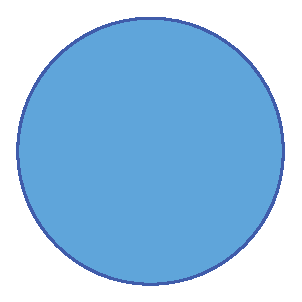
\includegraphics[width=50mm]{image.eps}}
    \end{center}
    \caption{図の例}
    \label{fig:sample1}
\end{figure}

ソースでは次のように記述している。

\begin{itembox}[l]{{\tt 03.tex}}
\begin{verbatim}
図は次のように出力される(図\ref{fig:sample1})。

\begin{figure}[htbp]
    \begin{center}
       \fbox{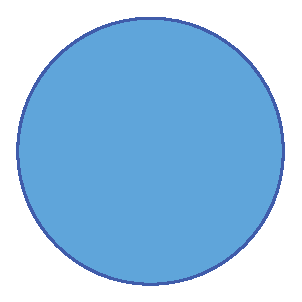
\includegraphics[width=40mm]{image.eps}}
    \end{center}
    \caption{図の例}
    \label{fig:sample1}
\end{figure}
\end{verbatim}
\end{itembox}

\verb|\begin{figure}[htbp]|  の{\tt htbp}は、表示位置の優先順位の設定。基本的に\LaTeX では、図の挿入位置は強制的には指定できない。いくつか候補を指定しておくと、候補のなかの優先度の高い順に、図を入れられるスペースがあるかどうかを調べて、入れられればそこに、入れられなければ次の候補のスペースを調べる、という処理が行われる。{\tt h}はこのコマンドを書いたその場所に、{\tt t}はページの一番上に、{\tt b}はページの一番下に、{\tt p}は画像だけ別ページに、それぞれ配置する。基本的には{\tt htbp}のように全部書いておけば問題ない。

\verb|\includegraphics| コマンドで、図のサイズと挿入するファイルを指定する。上の例ではサイズは {\tt width=50mm} として幅を指定したけれど、ここは他にも {\tt height=30mm} として高さを指定してもよいし、{\tt scale=0.5} として拡大率を指定してもよい。画像は最近の \LaTeX 環境であれば{\tt *.eps}以外でも使える。ただし、{\tt bb} (Bounding Box) として画像の大きさを指定する必要があることも多い。
以下はJPEG画像を使用する例。

\begin{itembox}[l]{{\tt 03.tex}}
\begin{verbatim}
\begin{figure}[htbp]
    \begin{center}
       \fbox{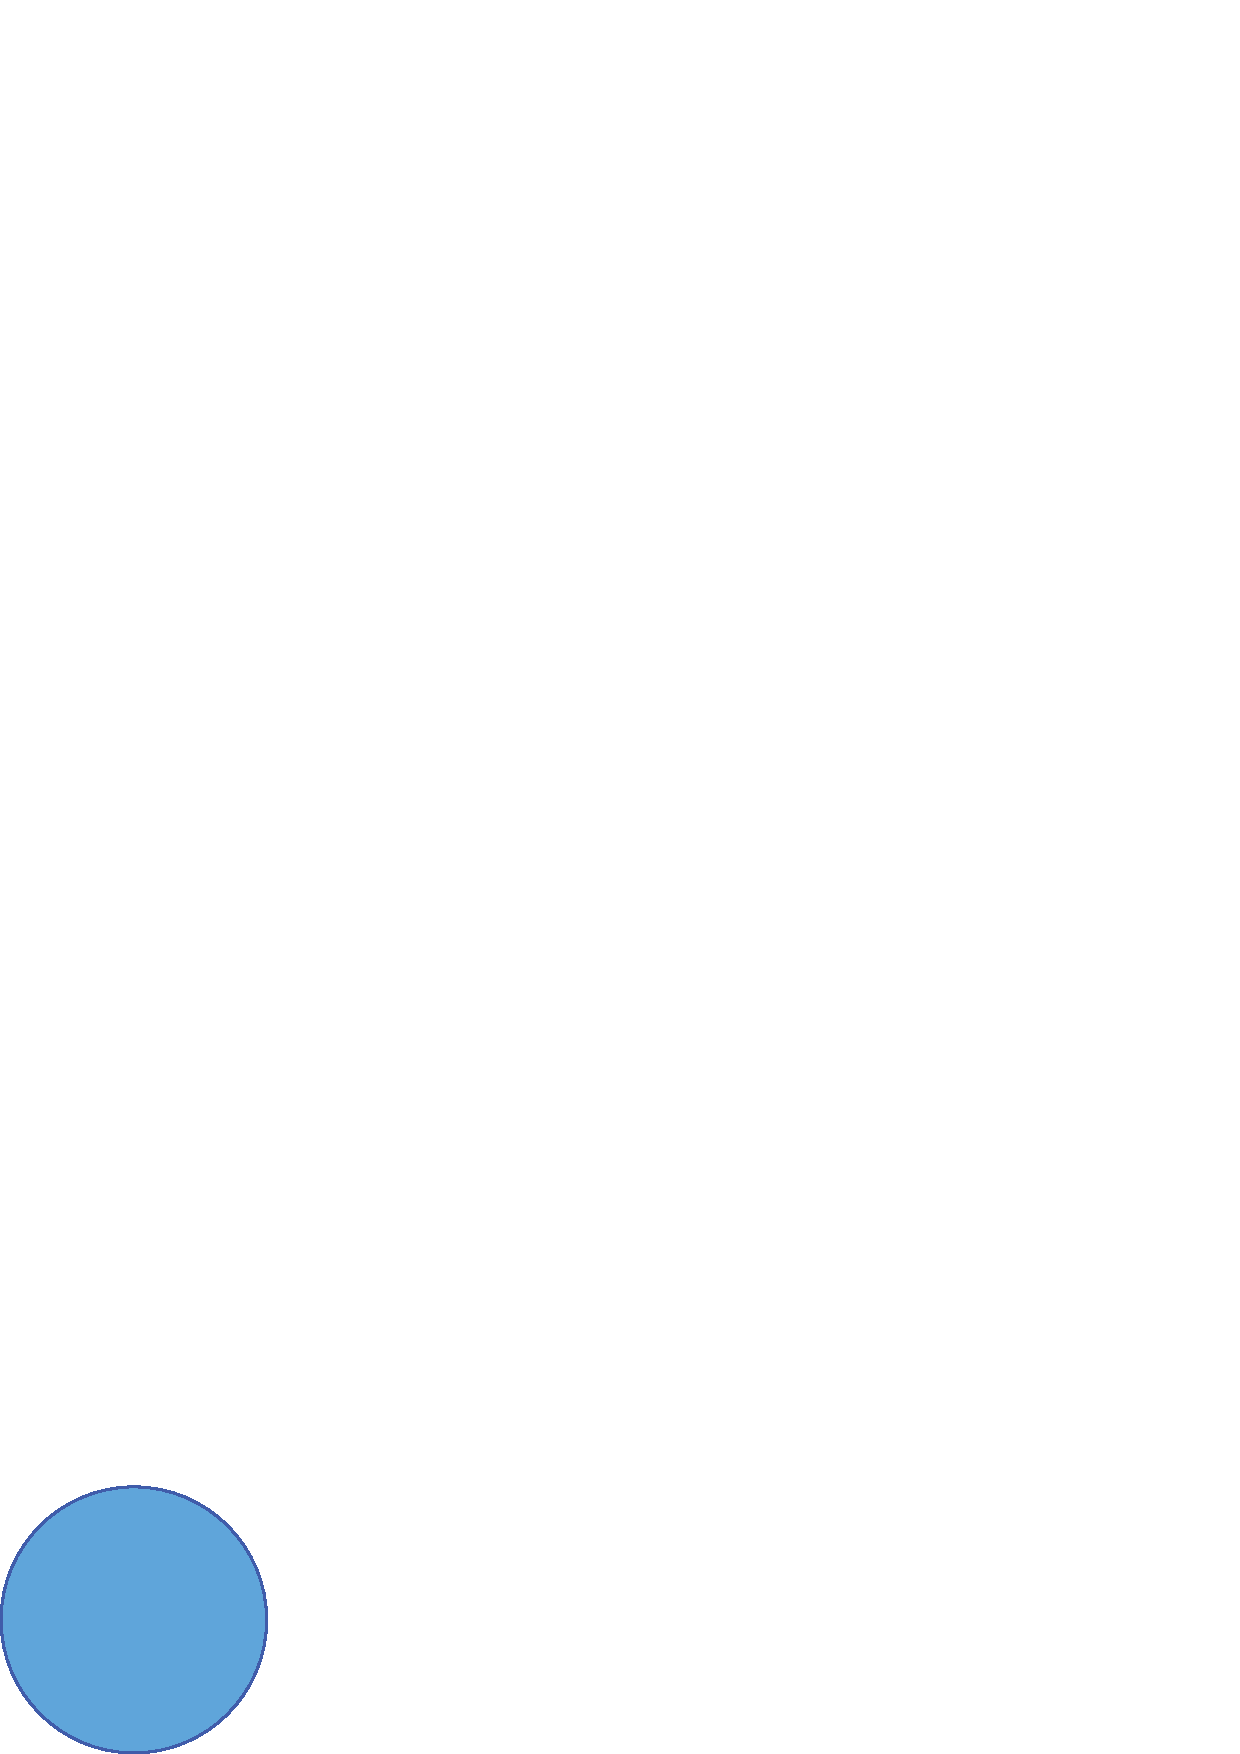
\includegraphics[width=40mm,bb=0 0 640 480]{image.jpg}}
    \end{center}
    \caption{図の例}
    \label{fig:sample1}
\end{figure}
\end{verbatim}
\end{itembox}

bbの指定は、上記のように{\tt *.tex} ファイルの中で指定してもいいが、
{\tt *.bb}ファイルを作っておく方法もある。
ターミナルで{\tt ebb}コマンドを使用すると{\tt *.bb}ファイルを簡単に作れる。


\begin{itembox}[l]{ebbコマンドの例}
\begin{verbatim}
% ebb image.jpg
\end{verbatim}
\end{itembox}


\verb|\includegraphics| を \verb|\fbox| に入れると、画像に枠を付けられる。

\verb|\caption| コマンドで図の見出しを指定できる。図の見出しは、図の下に表記するので注意。ここで指定した見出しが、図の目次に表示される。

\verb|\label| コマンドでは図の参照用ラベルを設定できる。本文中、\verb|\ref| コマンドで参照用ラベルを指定すると、対応した図の番号が自動的に挿入される。これも目次や参考文献と同様、最低二回のコンパイルが必要なので注意。

図を二つ横に並べたい場合は、次のように書く(図\ref{fig:sample2}、図\ref{fig:sample3})。

\begin{figure}[htbp]
  \begin{minipage}{0.5\hsize}
    \begin{center}
       \fbox{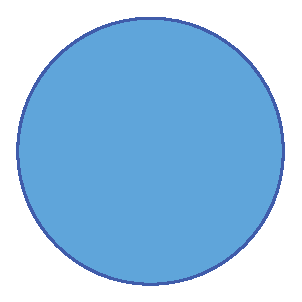
\includegraphics[width=40mm]{image.eps}}
    \end{center}
    \caption{図を並べる例1}
    \label{fig:sample2}
  \end{minipage}
  \begin{minipage}{0.5\hsize}
    \begin{center}
       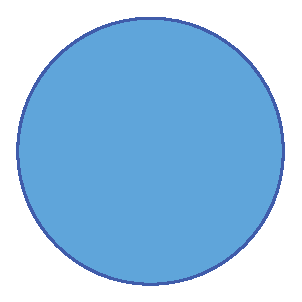
\includegraphics[width=40mm]{image.eps}
    \end{center}
    \caption{図を並べる例2、枠なし}
    \label{fig:sample3}
  \end{minipage}
\end{figure}

\begin{itembox}[l]{{\tt 03.tex}}
\begin{verbatim}
図を二つ横に並べたい場合は、次のように書く(図\ref{fig:sample2}、図\ref{fig:sample3})。

\begin{figure}[htbp]
  \begin{minipage}{0.5\hsize}
    \begin{center}
       \fbox{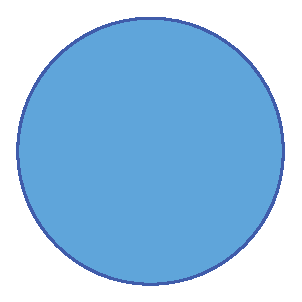
\includegraphics[width=40mm]{image.eps}}
    \end{center}
    \caption{図を並べる例1}
    \label{fig:sample2}
  \end{minipage}
  \begin{minipage}{0.5\hsize}
    \begin{center}
       \fbox{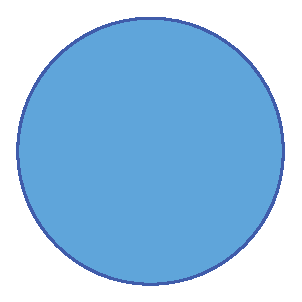
\includegraphics[width=40mm]{image.eps}}
    \end{center}
    \caption{図を並べる例2}
    \label{fig:sample3}
  \end{minipage}
\end{figure}
\end{verbatim}
\end{itembox}


\subsection{表}

表は次のように出力される(表\ref{tb:sample1})。

\begin{table}[htbp]
  \caption{表の例}
  \label{tb:sample1}
  \begin{center}
  \begin{tabular}{l|c|r}
    \hline
    種類	&味&評価\\\hline\hline
    ドラ焼き&甘い&好き\\\hline
    メロンパン&カリもふ&好き\\\hline
    クリームパン&神&すごく好き\\\hline
  \end{tabular}\end{center}
\end{table}

ソースでは次のようになっている。

\begin{itembox}[l]{{\tt 03.tex}}
\begin{verbatim}
表は次のように出力される(表\ref{tb:sample1})。

\begin{table}[htbp]
  \caption{表の例}
  \label{tb:sample1}
  \begin{center}
  \begin{tabular}{l|c|r}
    \hline
    種類	&味&評価\\\hline\hline
    ドラ焼き&甘い&好き\\\hline
    メロンパン&カリもふ&好き\\\hline
    クリームパン&神&すごく好き\\\hline
  \end{tabular}\end{center}
\end{table}
\end{verbatim}
\end{itembox}

{\tt htbp}や \verb|\caption| と \verb|\label| は図と同様。ただし表のタイトルは表の上に書く。

\verb|\begin{tabular}{l|{\tt \textbar}{\tt c}{\tt \textbar}\verb|r}|で横方向のセルを指定する。{\tt c}は中央揃え、{\tt l}は左揃え、{\tt r}は右揃えのセルを作る。{\tt \textbar}は垂直方向の罫線を表す。{\tt c}か{\tt l}か{\tt r}を必要なセルの数だけ並べて、セルの間に罫線が必要なら{\tt \textbar}を入れればよい。

セルの中の文字は、{\tt \&}で区切って並べる。行と行は \verb|\\| で区切る。水平方向の罫線が必要なら、\verb|\hline| を書く。

水平方向や垂直方向のセルの結合もできる。例を示すので、くわしくはぐぐろう。説明がめんどう。\verb|\multirow|、\verb|\multicolumn|、\verb|\cline| を使うとできる。

\begin{table}[htbp]
  \caption{セルを結合した例}
  \label{tb:sample2}
  \begin{center}
  \begin{tabular}{c|c|c}
    \hline
    ほげ&ふー&ばー\\\hline\hline
    \multirow{2}{*}{ほげほげ}&\multicolumn{2}{c}{ふーふー} \\\cline{2-3}
    &ふーふーふー&ばーばーばー\\\hline
  \end{tabular}
  \end{center}
\end{table}

\begin{itembox}[l]{{\tt 03.tex}}
\begin{verbatim}
\begin{table}[htbp]
  \caption{セルを結合した例}
  \label{tb:sample2}
  \begin{center}
  \begin{tabular}{c|c|c}
    \hline
    ほげ&ふー&ばー\\\hline\hline
    \multirow{2}{*}{ほげほげ}&\multicolumn{2}{c}{ふーふー} \\\cline{2-3}
    &ふーふーふー&ばーばーばー\\\hline
  \end{tabular}
  \end{center}
\end{table}
\end{verbatim}
\end{itembox}


\subsection{脚注}

脚注は \verb|\footnote| コマンドを使う。例えばこんな感じ\footnote{ページの下に小さく説明を出せる}。

\begin{itembox}[l]{{\tt 03.tex}}
\begin{verbatim}
例えばこんな感じ\footnote{ページの下に小さく説明を出せる}。
\end{verbatim}
\end{itembox}

\section{その他のコマンド}

ぐぐる\footnote{http://www.google.co.jp/}。

特殊なことは何もしていないテンプレートなので、ぐぐって出たことはだいたいそのまま何でも使える。

あるいは、このファイル自体も\LaTeX で書かれているわけだから、これの{\tt *.tex}を見るのもよいかもしれない。
	% 本文3
\chapter{結論}
\label{chap:conclusion}

この章では、結論らしいことをかく。

\section{まとめ}

\LaTeX の環境さえあればスタンダードな体裁の論文がたぶんだれでも作れる程度のテンプレートにはなっているはず。がんばって卒業しよう。


\section{大事なこと}

箇条書きで列挙する。

\begin{itemize}
 \item ぐぐる。これは単なる\LaTeX だし、\LaTeX はもう枯れた技術だから、調べれば文献はいくらでもある。
 \item 先生を頼る。
 \item 単位をきちんとる。
 \item 卒業する。
\end{itemize}


	% 本文4
\end{verbatim}
\end{itembox}

目次に続いて、論文のメイン、本文を記述する。アブストラクトと同様で、{\tt main.tex}に直接書くか、\verb|\include| コマンドを利用して別に用意したファイルを{\tt include}する。

本文の書き方は、第\ref{chap:latex}章で詳しく説明する。


\subsection{謝辞の出力}

\begin{itembox}[l]{{\tt main.tex}}
\begin{verbatim}
\begin{acknowledgment}

このテンプレートを改造するにあたって、@kurokoboとインターネット上のいくつかの修士論文などを参考にしました。感謝いたします。

\end{acknowledgment}
	% 謝辞。要独自コマンド、include先参照のこと
\end{verbatim}
\end{itembox}

本文のあとには、謝辞を出力する。\verb|begin{acknowledgment}| から \verb|end{acknowledgment}| の間に書いた文章が、謝辞として独立したページに出力される。アブストラクトや本文と同じで、{\tt main.tex}に直接書いてもよいし、\verb|\include| コマンドを利用して{\tt include}してもよい。


\subsection{参考文献の出力}

\begin{itembox}[l]{{\tt main.tex}}
\begin{verbatim}

\begin{bib}[100]

\bibliography{main}

\end{bib}
	% 参考文献。要独自コマンド、include先参照のこと
\end{verbatim}
\end{itembox}

謝辞に続いて、参考文献を出力する。

参考文献リストは、\verb|\begin{bib}| から \verb|\end{bib}| の間に、\verb|\bibitem| コマンドを使って書く。

BibTeXを使う場合は、以下のようにする。

\begin{itembox}[l]{{\tt 91\_bibliography.tex}}
\begin{verbatim}
\begin{bib}[100]
\bibliography{main}
\end{bib}
\end{verbatim}
\end{itembox}

こうすると、\verb|main.bib|から使用した参考文献のみを抽出して出力してくれる。\verb|main.bib|の中身は以下のようになっていて、気の利いた論文検索サイトであればBibTeXをコピペできるようになっているので簡単に作れるはず。


\begin{itembox}[l]{{\tt 91\_bibliography.tex}}
\begin{verbatim}
@article{hoge09,
    author  = "ほげ山太郎 and ほげ山次郎",
    yomi    = "ほげやまたろう",
    title   = "ほげほげ理論のHCI分野への応用",
    journal = "ほげほげ学会論文誌",
    volume  = "31",
    number  = "3",
    pages   = "194-201",
    year    = "2009",
}
@inproceedings{hoge08,
    author     = "Taro Hogeyama and Jiro Hogeyama",
    title      = "The Theory of Hoge",
    booktitle  = "The Proceedings of The Hoge Society",
    year       = "2008"
}
\end{verbatim}
\end{itembox}


以下は、BibTeXを使わないで手で書く例。

\begin{itembox}[l]{{\tt 91\_bibliography.tex}}
\begin{verbatim}
@article{hoge09,
    author  = "ほげ山太郎 and ほげ山次郎",
    yomi    = "ほげやまたろう",
    title   = "ほげほげ理論のHCI分野への応用",
    journal = "ほげほげ学会論文誌",
    volume  = "31",
    number  = "3",
    pages   = "194-201",
    year    = "2009",
}
@inproceedings{hoge08,
    author     = "Taro Hogeyama and Jiro Hogeyama",
    title      = "The Theory of Hoge",
    booktitle  = "The Proceedings of The Hoge Society",
    year       = "2008"
}
\end{verbatim}
\end{itembox}


英語の文献の場合、慣例的に書誌名をイタリック体にすることが多いらしい。

\begin{itembox}[l]{{\tt 91\_bibliography.tex}}
\begin{verbatim}
\begin{bib}[100]
\begin{thebibliography}{#1}
% \bibitem{参照用名称}
%   著者名: 
%   \newblock 文献名,
%   \newblock 書誌情報,出版年.

\bibitem{hoge09}
  ほげ山太郎,ほげ山次郎:
  \newblock ほげほげ理論のHCI分野への応用,
  \newblock ほげほげ学会論文誌,Vol.31,No.3,pp.194-201,2009.

\bibitem{hoge08}
  Taro Hogeyama, Jiro Hogeyama:
  \newblock The Theory of Hoge,
  \newblock {\it The Proceedings of The Hoge Society}, 2008.
\end{thebibliography}
\end{bib}
\end{verbatim}
\end{itembox}

\verb|\bibitem| コマンド中、参照用名称は、本文から参考文献を参照するときに使うので、忘れずに書いておく。参照文献を本文中に参照するときには、\verb|\cite{参照用名称}| のように書けばよい。例えば、この文の末尾には \verb|\cite{hoge09}| と書いてあるので、自動で対応する番号が振られる\cite{hoge09}\cite{hoge08}。

参考文献リストの番号付けと、本文で参照したときの番号の挿入は、全部が自動で行われる。ただしこれも、第\ref{sec:toc}節で説明した目次の出力と同じで、一時ファイルを生成してからの挿入なので、正しく出力するには最低でも二回のコンパイルが必要。BibTeXを使用する場合は、\verb|platex|コマンドのあと\verb|pbibtex|コマンドを実行し、さらに2回\verb|platex|コマンドを実行するといいらしい。



\subsection{付録の出力}

\begin{itembox}[l]{{\tt main.tex}}
\begin{verbatim}
\appendix
\chapter{付録の例}

付録を無理矢理出力させるため、てきとうなことを書く。

\section{ほげ}

コマンドは本文と一緒。

\subsection{ふー}

本文と一緒。

\section{ほげほげ}

本文と一緒。

\subsection{ふーふー}

本文と一緒。
		% 付録
\end{verbatim}
\end{itembox}

必要であれば、論文の最後には付録を出力する。

\verb|\appendix| コマンド以降に書いたものは、すべて付録として扱われる。付録部分の書き方は通常の本文とまったく同じで、\verb|\appendix| コマンド以降に書くだけで勝手に付録用の体裁で出力される。
	% 本文2
\chapter{\LaTeX の書き方}
\label{chap:latex}

この章では、よく使う\LaTeX のコマンドを説明する。足りない部分はぐぐればだいたいわかると思う。最初に書いておくと、数式を書く方法は、ぼく自身使わなかったので書いていない。ぼくのいた研究室でごりごり数式をたくさん書く必要のあるひとは、研究の種類からするとあまり居ない気がする。

\section{主なコマンド}

\subsection{章と節}

文書構造を明確にする大事なもの。目次はこれらのコマンドをもとに作られる。例えば、この第\ref{chap:latex}章の冒頭部分はこのようなソースで書かれている。

\begin{itembox}[l]{{\tt 03.tex}}
\begin{verbatim}
\chapter{\LaTeX の書き方}
\label{chap:latex}

この章では、よく使う\LaTeX のコマンドを説明する。(略)

\section{主なコマンド}

\subsection{章と節}

文書構造を明確にする大事なもの。目次はこれらのコマンドをもとに作られる。例えば、この第\ref{chap:latex}章の冒頭部分はこのようなソースで書かれている。
\end{verbatim}
\end{itembox}

章は \verb|\chapter{見出し}|、節は \verb|\section{見出し}|、小節は \verb|\subsection{見出し}|、小々節は \verb|\subsubsection{見出し}| を使う。表\ref{tb:chap}に一覧する。

\begin{table}[htbp]
  \caption{章と節のコマンド}
  \label{tb:chap}
  \begin{center}\begin{tabular}{c|c}
    \hline
    コマンド&用途\\\hline\hline
    \verb|\chapter{見出し}|&章\\\hline
    \verb|\section{見出し}|&節\\\hline
    \verb|\subsection{見出し}|&小節\\\hline
    \verb|\subsubsection{見出し}|&小々節\\\hline
    \end{tabular}\end{center}
\end{table}

\subsubsection{小々節見出しサンプルその1}

小々節は上のように \verb|\subsubsection{タイトル}| で書けるけれど、あまり文書の階層構造が深いことは望ましくないので、多用しなければならないようなら文書構造を見直したほうがよいと思う。

\subsubsection{小々節見出しサンプルその2}

小々節は、章や節、小節のように {\tt N.N.N} といった番号ではなくて、括弧付きの番号で出力される。かつ、目次には出力されない。

\subsection{図}

図は次のように出力される(図\ref{fig:sample1})。

\begin{figure}[htbp]
    \begin{center}
       \fbox{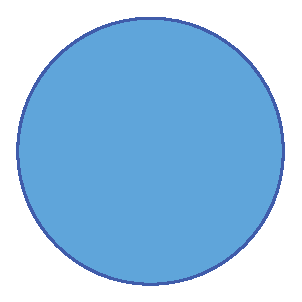
\includegraphics[width=50mm]{image.eps}}
    \end{center}
    \caption{図の例}
    \label{fig:sample1}
\end{figure}

ソースでは次のように記述している。

\begin{itembox}[l]{{\tt 03.tex}}
\begin{verbatim}
図は次のように出力される(図\ref{fig:sample1})。

\begin{figure}[htbp]
    \begin{center}
       \fbox{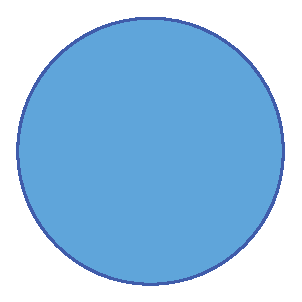
\includegraphics[width=40mm]{image.eps}}
    \end{center}
    \caption{図の例}
    \label{fig:sample1}
\end{figure}
\end{verbatim}
\end{itembox}

\verb|\begin{figure}[htbp]|  の{\tt htbp}は、表示位置の優先順位の設定。基本的に\LaTeX では、図の挿入位置は強制的には指定できない。いくつか候補を指定しておくと、候補のなかの優先度の高い順に、図を入れられるスペースがあるかどうかを調べて、入れられればそこに、入れられなければ次の候補のスペースを調べる、という処理が行われる。{\tt h}はこのコマンドを書いたその場所に、{\tt t}はページの一番上に、{\tt b}はページの一番下に、{\tt p}は画像だけ別ページに、それぞれ配置する。基本的には{\tt htbp}のように全部書いておけば問題ない。

\verb|\includegraphics| コマンドで、図のサイズと挿入するファイルを指定する。上の例ではサイズは {\tt width=50mm} として幅を指定したけれど、ここは他にも {\tt height=30mm} として高さを指定してもよいし、{\tt scale=0.5} として拡大率を指定してもよい。画像は最近の \LaTeX 環境であれば{\tt *.eps}以外でも使える。ただし、{\tt bb} (Bounding Box) として画像の大きさを指定する必要があることも多い。
以下はJPEG画像を使用する例。

\begin{itembox}[l]{{\tt 03.tex}}
\begin{verbatim}
\begin{figure}[htbp]
    \begin{center}
       \fbox{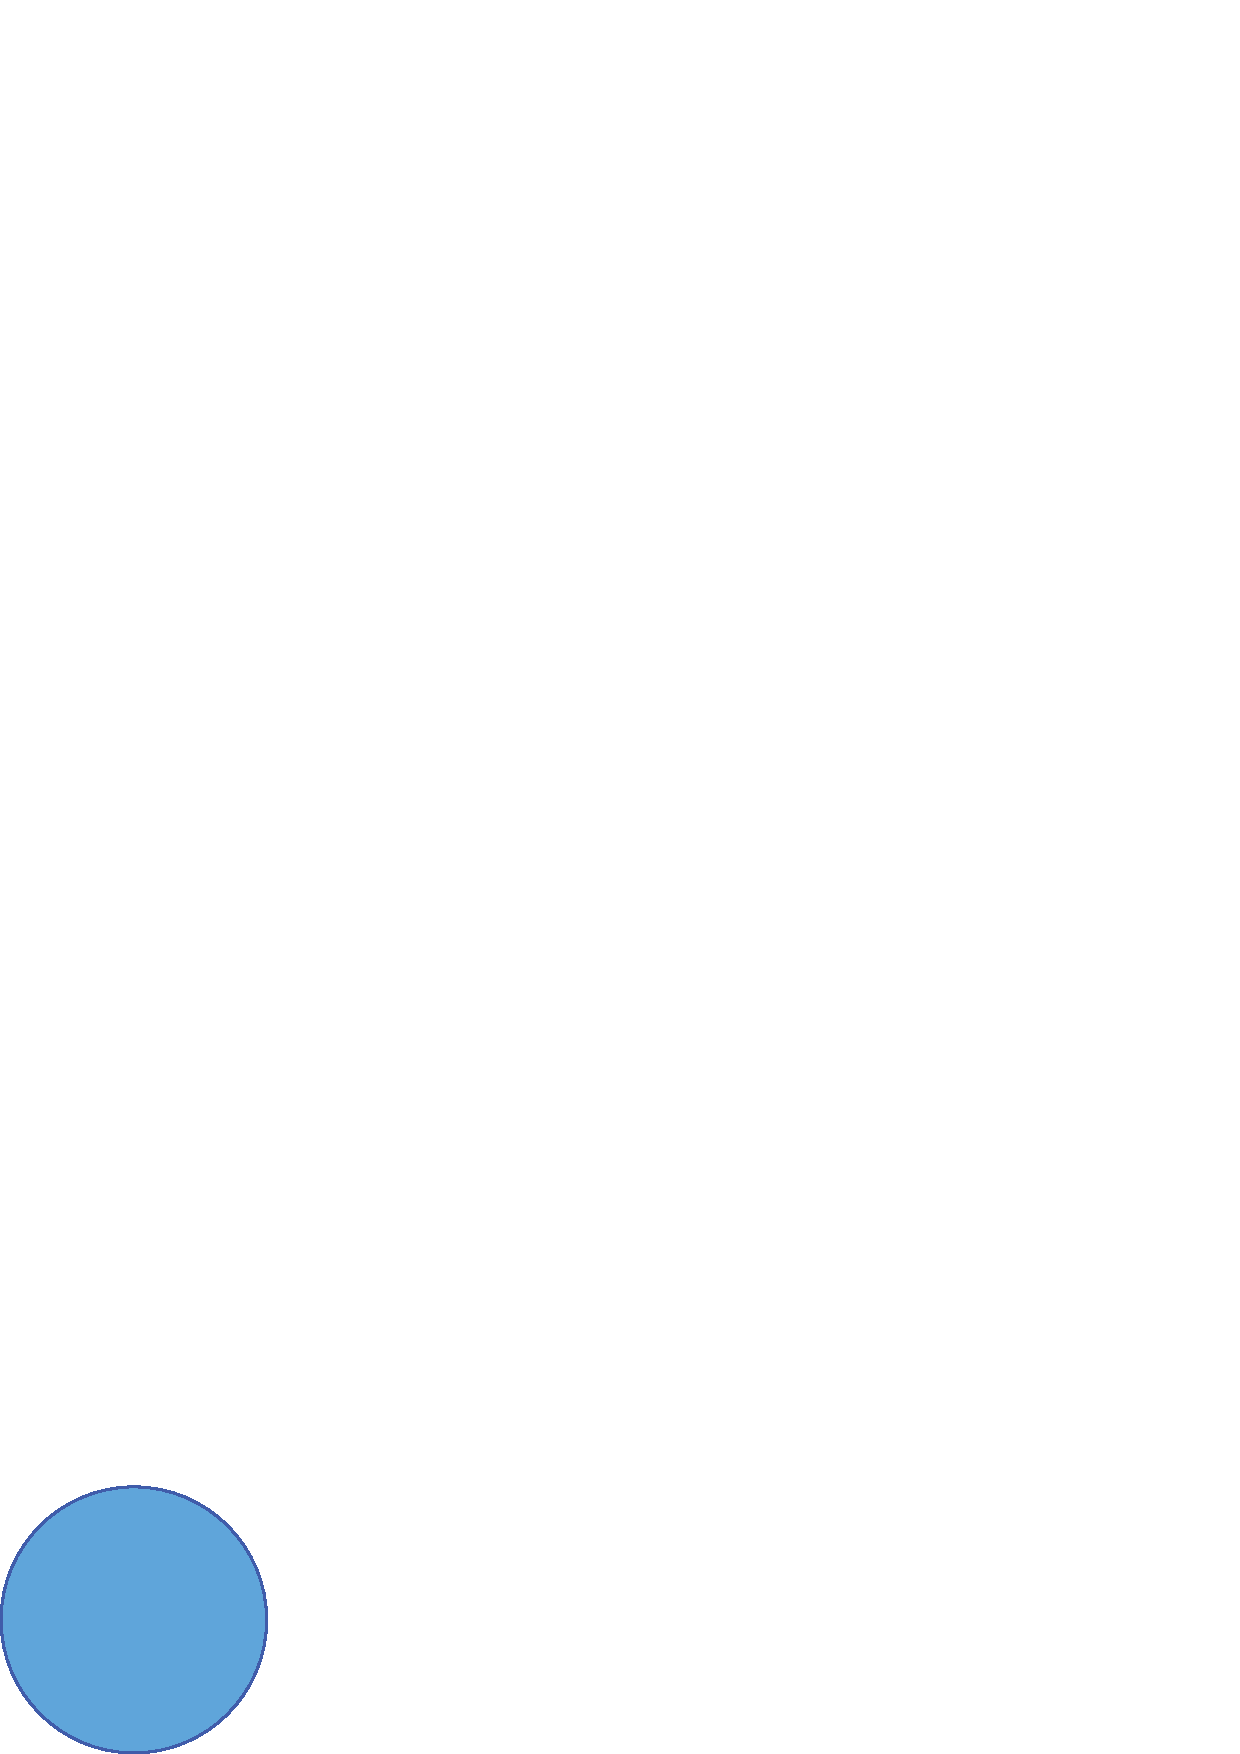
\includegraphics[width=40mm,bb=0 0 640 480]{image.jpg}}
    \end{center}
    \caption{図の例}
    \label{fig:sample1}
\end{figure}
\end{verbatim}
\end{itembox}

bbの指定は、上記のように{\tt *.tex} ファイルの中で指定してもいいが、
{\tt *.bb}ファイルを作っておく方法もある。
ターミナルで{\tt ebb}コマンドを使用すると{\tt *.bb}ファイルを簡単に作れる。


\begin{itembox}[l]{ebbコマンドの例}
\begin{verbatim}
% ebb image.jpg
\end{verbatim}
\end{itembox}


\verb|\includegraphics| を \verb|\fbox| に入れると、画像に枠を付けられる。

\verb|\caption| コマンドで図の見出しを指定できる。図の見出しは、図の下に表記するので注意。ここで指定した見出しが、図の目次に表示される。

\verb|\label| コマンドでは図の参照用ラベルを設定できる。本文中、\verb|\ref| コマンドで参照用ラベルを指定すると、対応した図の番号が自動的に挿入される。これも目次や参考文献と同様、最低二回のコンパイルが必要なので注意。

図を二つ横に並べたい場合は、次のように書く(図\ref{fig:sample2}、図\ref{fig:sample3})。

\begin{figure}[htbp]
  \begin{minipage}{0.5\hsize}
    \begin{center}
       \fbox{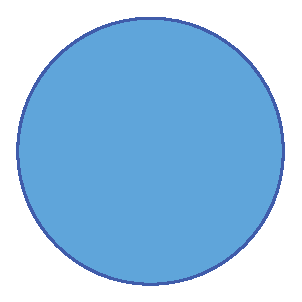
\includegraphics[width=40mm]{image.eps}}
    \end{center}
    \caption{図を並べる例1}
    \label{fig:sample2}
  \end{minipage}
  \begin{minipage}{0.5\hsize}
    \begin{center}
       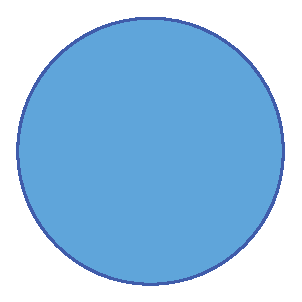
\includegraphics[width=40mm]{image.eps}
    \end{center}
    \caption{図を並べる例2、枠なし}
    \label{fig:sample3}
  \end{minipage}
\end{figure}

\begin{itembox}[l]{{\tt 03.tex}}
\begin{verbatim}
図を二つ横に並べたい場合は、次のように書く(図\ref{fig:sample2}、図\ref{fig:sample3})。

\begin{figure}[htbp]
  \begin{minipage}{0.5\hsize}
    \begin{center}
       \fbox{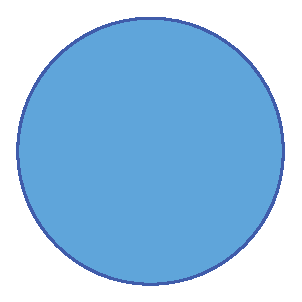
\includegraphics[width=40mm]{image.eps}}
    \end{center}
    \caption{図を並べる例1}
    \label{fig:sample2}
  \end{minipage}
  \begin{minipage}{0.5\hsize}
    \begin{center}
       \fbox{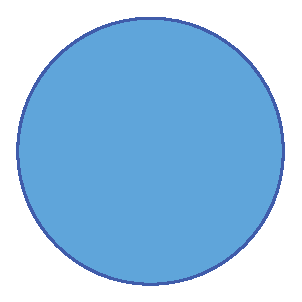
\includegraphics[width=40mm]{image.eps}}
    \end{center}
    \caption{図を並べる例2}
    \label{fig:sample3}
  \end{minipage}
\end{figure}
\end{verbatim}
\end{itembox}


\subsection{表}

表は次のように出力される(表\ref{tb:sample1})。

\begin{table}[htbp]
  \caption{表の例}
  \label{tb:sample1}
  \begin{center}
  \begin{tabular}{l|c|r}
    \hline
    種類	&味&評価\\\hline\hline
    ドラ焼き&甘い&好き\\\hline
    メロンパン&カリもふ&好き\\\hline
    クリームパン&神&すごく好き\\\hline
  \end{tabular}\end{center}
\end{table}

ソースでは次のようになっている。

\begin{itembox}[l]{{\tt 03.tex}}
\begin{verbatim}
表は次のように出力される(表\ref{tb:sample1})。

\begin{table}[htbp]
  \caption{表の例}
  \label{tb:sample1}
  \begin{center}
  \begin{tabular}{l|c|r}
    \hline
    種類	&味&評価\\\hline\hline
    ドラ焼き&甘い&好き\\\hline
    メロンパン&カリもふ&好き\\\hline
    クリームパン&神&すごく好き\\\hline
  \end{tabular}\end{center}
\end{table}
\end{verbatim}
\end{itembox}

{\tt htbp}や \verb|\caption| と \verb|\label| は図と同様。ただし表のタイトルは表の上に書く。

\verb|\begin{tabular}{l|{\tt \textbar}{\tt c}{\tt \textbar}\verb|r}|で横方向のセルを指定する。{\tt c}は中央揃え、{\tt l}は左揃え、{\tt r}は右揃えのセルを作る。{\tt \textbar}は垂直方向の罫線を表す。{\tt c}か{\tt l}か{\tt r}を必要なセルの数だけ並べて、セルの間に罫線が必要なら{\tt \textbar}を入れればよい。

セルの中の文字は、{\tt \&}で区切って並べる。行と行は \verb|\\| で区切る。水平方向の罫線が必要なら、\verb|\hline| を書く。

水平方向や垂直方向のセルの結合もできる。例を示すので、くわしくはぐぐろう。説明がめんどう。\verb|\multirow|、\verb|\multicolumn|、\verb|\cline| を使うとできる。

\begin{table}[htbp]
  \caption{セルを結合した例}
  \label{tb:sample2}
  \begin{center}
  \begin{tabular}{c|c|c}
    \hline
    ほげ&ふー&ばー\\\hline\hline
    \multirow{2}{*}{ほげほげ}&\multicolumn{2}{c}{ふーふー} \\\cline{2-3}
    &ふーふーふー&ばーばーばー\\\hline
  \end{tabular}
  \end{center}
\end{table}

\begin{itembox}[l]{{\tt 03.tex}}
\begin{verbatim}
\begin{table}[htbp]
  \caption{セルを結合した例}
  \label{tb:sample2}
  \begin{center}
  \begin{tabular}{c|c|c}
    \hline
    ほげ&ふー&ばー\\\hline\hline
    \multirow{2}{*}{ほげほげ}&\multicolumn{2}{c}{ふーふー} \\\cline{2-3}
    &ふーふーふー&ばーばーばー\\\hline
  \end{tabular}
  \end{center}
\end{table}
\end{verbatim}
\end{itembox}


\subsection{脚注}

脚注は \verb|\footnote| コマンドを使う。例えばこんな感じ\footnote{ページの下に小さく説明を出せる}。

\begin{itembox}[l]{{\tt 03.tex}}
\begin{verbatim}
例えばこんな感じ\footnote{ページの下に小さく説明を出せる}。
\end{verbatim}
\end{itembox}

\section{その他のコマンド}

ぐぐる\footnote{http://www.google.co.jp/}。

特殊なことは何もしていないテンプレートなので、ぐぐって出たことはだいたいそのまま何でも使える。

あるいは、このファイル自体も\LaTeX で書かれているわけだから、これの{\tt *.tex}を見るのもよいかもしれない。
	% 本文3
\chapter{結論}
\label{chap:conclusion}

この章では、結論らしいことをかく。

\section{まとめ}

\LaTeX の環境さえあればスタンダードな体裁の論文がたぶんだれでも作れる程度のテンプレートにはなっているはず。がんばって卒業しよう。


\section{大事なこと}

箇条書きで列挙する。

\begin{itemize}
 \item ぐぐる。これは単なる\LaTeX だし、\LaTeX はもう枯れた技術だから、調べれば文献はいくらでもある。
 \item 先生を頼る。
 \item 単位をきちんとる。
 \item 卒業する。
\end{itemize}


	% 本文4
\end{verbatim}
\end{itembox}

目次に続いて、論文のメイン、本文を記述する。アブストラクトと同様で、{\tt main.tex}に直接書くか、\verb|\include| コマンドを利用して別に用意したファイルを{\tt include}する。

本文の書き方は、第\ref{chap:latex}章で詳しく説明する。


\subsection{謝辞の出力}

\begin{itembox}[l]{{\tt main.tex}}
\begin{verbatim}
\begin{acknowledgment}

このテンプレートを改造するにあたって、@kurokoboとインターネット上のいくつかの修士論文などを参考にしました。感謝いたします。

\end{acknowledgment}
	% 謝辞。要独自コマンド、include先参照のこと
\end{verbatim}
\end{itembox}

本文のあとには、謝辞を出力する。\verb|begin{acknowledgment}| から \verb|end{acknowledgment}| の間に書いた文章が、謝辞として独立したページに出力される。アブストラクトや本文と同じで、{\tt main.tex}に直接書いてもよいし、\verb|\include| コマンドを利用して{\tt include}してもよい。


\subsection{参考文献の出力}

\begin{itembox}[l]{{\tt main.tex}}
\begin{verbatim}

\begin{bib}[100]

\bibliography{main}

\end{bib}
	% 参考文献。要独自コマンド、include先参照のこと
\end{verbatim}
\end{itembox}

謝辞に続いて、参考文献を出力する。

参考文献リストは、\verb|\begin{bib}| から \verb|\end{bib}| の間に、\verb|\bibitem| コマンドを使って書く。

BibTeXを使う場合は、以下のようにする。

\begin{itembox}[l]{{\tt 91\_bibliography.tex}}
\begin{verbatim}
\begin{bib}[100]
\bibliography{main}
\end{bib}
\end{verbatim}
\end{itembox}

こうすると、\verb|main.bib|から使用した参考文献のみを抽出して出力してくれる。\verb|main.bib|の中身は以下のようになっていて、気の利いた論文検索サイトであればBibTeXをコピペできるようになっているので簡単に作れるはず。


\begin{itembox}[l]{{\tt 91\_bibliography.tex}}
\begin{verbatim}
@article{hoge09,
    author  = "ほげ山太郎 and ほげ山次郎",
    yomi    = "ほげやまたろう",
    title   = "ほげほげ理論のHCI分野への応用",
    journal = "ほげほげ学会論文誌",
    volume  = "31",
    number  = "3",
    pages   = "194-201",
    year    = "2009",
}
@inproceedings{hoge08,
    author     = "Taro Hogeyama and Jiro Hogeyama",
    title      = "The Theory of Hoge",
    booktitle  = "The Proceedings of The Hoge Society",
    year       = "2008"
}
\end{verbatim}
\end{itembox}


以下は、BibTeXを使わないで手で書く例。

\begin{itembox}[l]{{\tt 91\_bibliography.tex}}
\begin{verbatim}
@article{hoge09,
    author  = "ほげ山太郎 and ほげ山次郎",
    yomi    = "ほげやまたろう",
    title   = "ほげほげ理論のHCI分野への応用",
    journal = "ほげほげ学会論文誌",
    volume  = "31",
    number  = "3",
    pages   = "194-201",
    year    = "2009",
}
@inproceedings{hoge08,
    author     = "Taro Hogeyama and Jiro Hogeyama",
    title      = "The Theory of Hoge",
    booktitle  = "The Proceedings of The Hoge Society",
    year       = "2008"
}
\end{verbatim}
\end{itembox}


英語の文献の場合、慣例的に書誌名をイタリック体にすることが多いらしい。

\begin{itembox}[l]{{\tt 91\_bibliography.tex}}
\begin{verbatim}
\begin{bib}[100]
\begin{thebibliography}{#1}
% \bibitem{参照用名称}
%   著者名: 
%   \newblock 文献名,
%   \newblock 書誌情報,出版年.

\bibitem{hoge09}
  ほげ山太郎,ほげ山次郎:
  \newblock ほげほげ理論のHCI分野への応用,
  \newblock ほげほげ学会論文誌,Vol.31,No.3,pp.194-201,2009.

\bibitem{hoge08}
  Taro Hogeyama, Jiro Hogeyama:
  \newblock The Theory of Hoge,
  \newblock {\it The Proceedings of The Hoge Society}, 2008.
\end{thebibliography}
\end{bib}
\end{verbatim}
\end{itembox}

\verb|\bibitem| コマンド中、参照用名称は、本文から参考文献を参照するときに使うので、忘れずに書いておく。参照文献を本文中に参照するときには、\verb|\cite{参照用名称}| のように書けばよい。例えば、この文の末尾には \verb|\cite{hoge09}| と書いてあるので、自動で対応する番号が振られる\cite{hoge09}\cite{hoge08}。

参考文献リストの番号付けと、本文で参照したときの番号の挿入は、全部が自動で行われる。ただしこれも、第\ref{sec:toc}節で説明した目次の出力と同じで、一時ファイルを生成してからの挿入なので、正しく出力するには最低でも二回のコンパイルが必要。BibTeXを使用する場合は、\verb|platex|コマンドのあと\verb|pbibtex|コマンドを実行し、さらに2回\verb|platex|コマンドを実行するといいらしい。



\subsection{付録の出力}

\begin{itembox}[l]{{\tt main.tex}}
\begin{verbatim}
\appendix
\chapter{付録の例}

付録を無理矢理出力させるため、てきとうなことを書く。

\section{ほげ}

コマンドは本文と一緒。

\subsection{ふー}

本文と一緒。

\section{ほげほげ}

本文と一緒。

\subsection{ふーふー}

本文と一緒。
		% 付録
\end{verbatim}
\end{itembox}

必要であれば、論文の最後には付録を出力する。

\verb|\appendix| コマンド以降に書いたものは、すべて付録として扱われる。付録部分の書き方は通常の本文とまったく同じで、\verb|\appendix| コマンド以降に書くだけで勝手に付録用の体裁で出力される。
  % 本文2
\chapter{\LaTeX の書き方}
\label{chap:latex}

この章では、よく使う\LaTeX のコマンドを説明する。足りない部分はぐぐればだいたいわかると思う。最初に書いておくと、数式を書く方法は、ぼく自身使わなかったので書いていない。ぼくのいた研究室でごりごり数式をたくさん書く必要のあるひとは、研究の種類からするとあまり居ない気がする。

\section{主なコマンド}

\subsection{章と節}

文書構造を明確にする大事なもの。目次はこれらのコマンドをもとに作られる。例えば、この第\ref{chap:latex}章の冒頭部分はこのようなソースで書かれている。

\begin{itembox}[l]{{\tt 03.tex}}
\begin{verbatim}
\chapter{\LaTeX の書き方}
\label{chap:latex}

この章では、よく使う\LaTeX のコマンドを説明する。(略)

\section{主なコマンド}

\subsection{章と節}

文書構造を明確にする大事なもの。目次はこれらのコマンドをもとに作られる。例えば、この第\ref{chap:latex}章の冒頭部分はこのようなソースで書かれている。
\end{verbatim}
\end{itembox}

章は \verb|\chapter{見出し}|、節は \verb|\section{見出し}|、小節は \verb|\subsection{見出し}|、小々節は \verb|\subsubsection{見出し}| を使う。表\ref{tb:chap}に一覧する。

\begin{table}[htbp]
  \caption{章と節のコマンド}
  \label{tb:chap}
  \begin{center}\begin{tabular}{c|c}
    \hline
    コマンド&用途\\\hline\hline
    \verb|\chapter{見出し}|&章\\\hline
    \verb|\section{見出し}|&節\\\hline
    \verb|\subsection{見出し}|&小節\\\hline
    \verb|\subsubsection{見出し}|&小々節\\\hline
    \end{tabular}\end{center}
\end{table}

\subsubsection{小々節見出しサンプルその1}

小々節は上のように \verb|\subsubsection{タイトル}| で書けるけれど、あまり文書の階層構造が深いことは望ましくないので、多用しなければならないようなら文書構造を見直したほうがよいと思う。

\subsubsection{小々節見出しサンプルその2}

小々節は、章や節、小節のように {\tt N.N.N} といった番号ではなくて、括弧付きの番号で出力される。かつ、目次には出力されない。

\subsection{図}

図は次のように出力される(図\ref{fig:sample1})。

\begin{figure}[htbp]
    \begin{center}
       \fbox{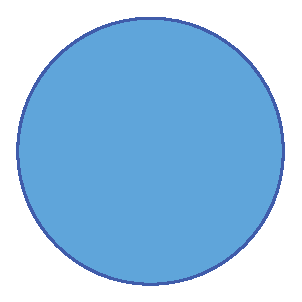
\includegraphics[width=50mm]{image.eps}}
    \end{center}
    \caption{図の例}
    \label{fig:sample1}
\end{figure}

ソースでは次のように記述している。

\begin{itembox}[l]{{\tt 03.tex}}
\begin{verbatim}
図は次のように出力される(図\ref{fig:sample1})。

\begin{figure}[htbp]
    \begin{center}
       \fbox{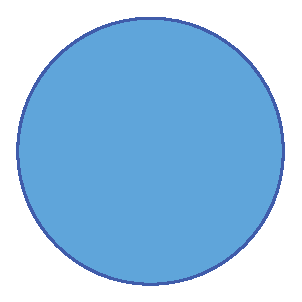
\includegraphics[width=40mm]{image.eps}}
    \end{center}
    \caption{図の例}
    \label{fig:sample1}
\end{figure}
\end{verbatim}
\end{itembox}

\verb|\begin{figure}[htbp]|  の{\tt htbp}は、表示位置の優先順位の設定。基本的に\LaTeX では、図の挿入位置は強制的には指定できない。いくつか候補を指定しておくと、候補のなかの優先度の高い順に、図を入れられるスペースがあるかどうかを調べて、入れられればそこに、入れられなければ次の候補のスペースを調べる、という処理が行われる。{\tt h}はこのコマンドを書いたその場所に、{\tt t}はページの一番上に、{\tt b}はページの一番下に、{\tt p}は画像だけ別ページに、それぞれ配置する。基本的には{\tt htbp}のように全部書いておけば問題ない。

\verb|\includegraphics| コマンドで、図のサイズと挿入するファイルを指定する。上の例ではサイズは {\tt width=50mm} として幅を指定したけれど、ここは他にも {\tt height=30mm} として高さを指定してもよいし、{\tt scale=0.5} として拡大率を指定してもよい。画像は最近の \LaTeX 環境であれば{\tt *.eps}以外でも使える。ただし、{\tt bb} (Bounding Box) として画像の大きさを指定する必要があることも多い。
以下はJPEG画像を使用する例。

\begin{itembox}[l]{{\tt 03.tex}}
\begin{verbatim}
\begin{figure}[htbp]
    \begin{center}
       \fbox{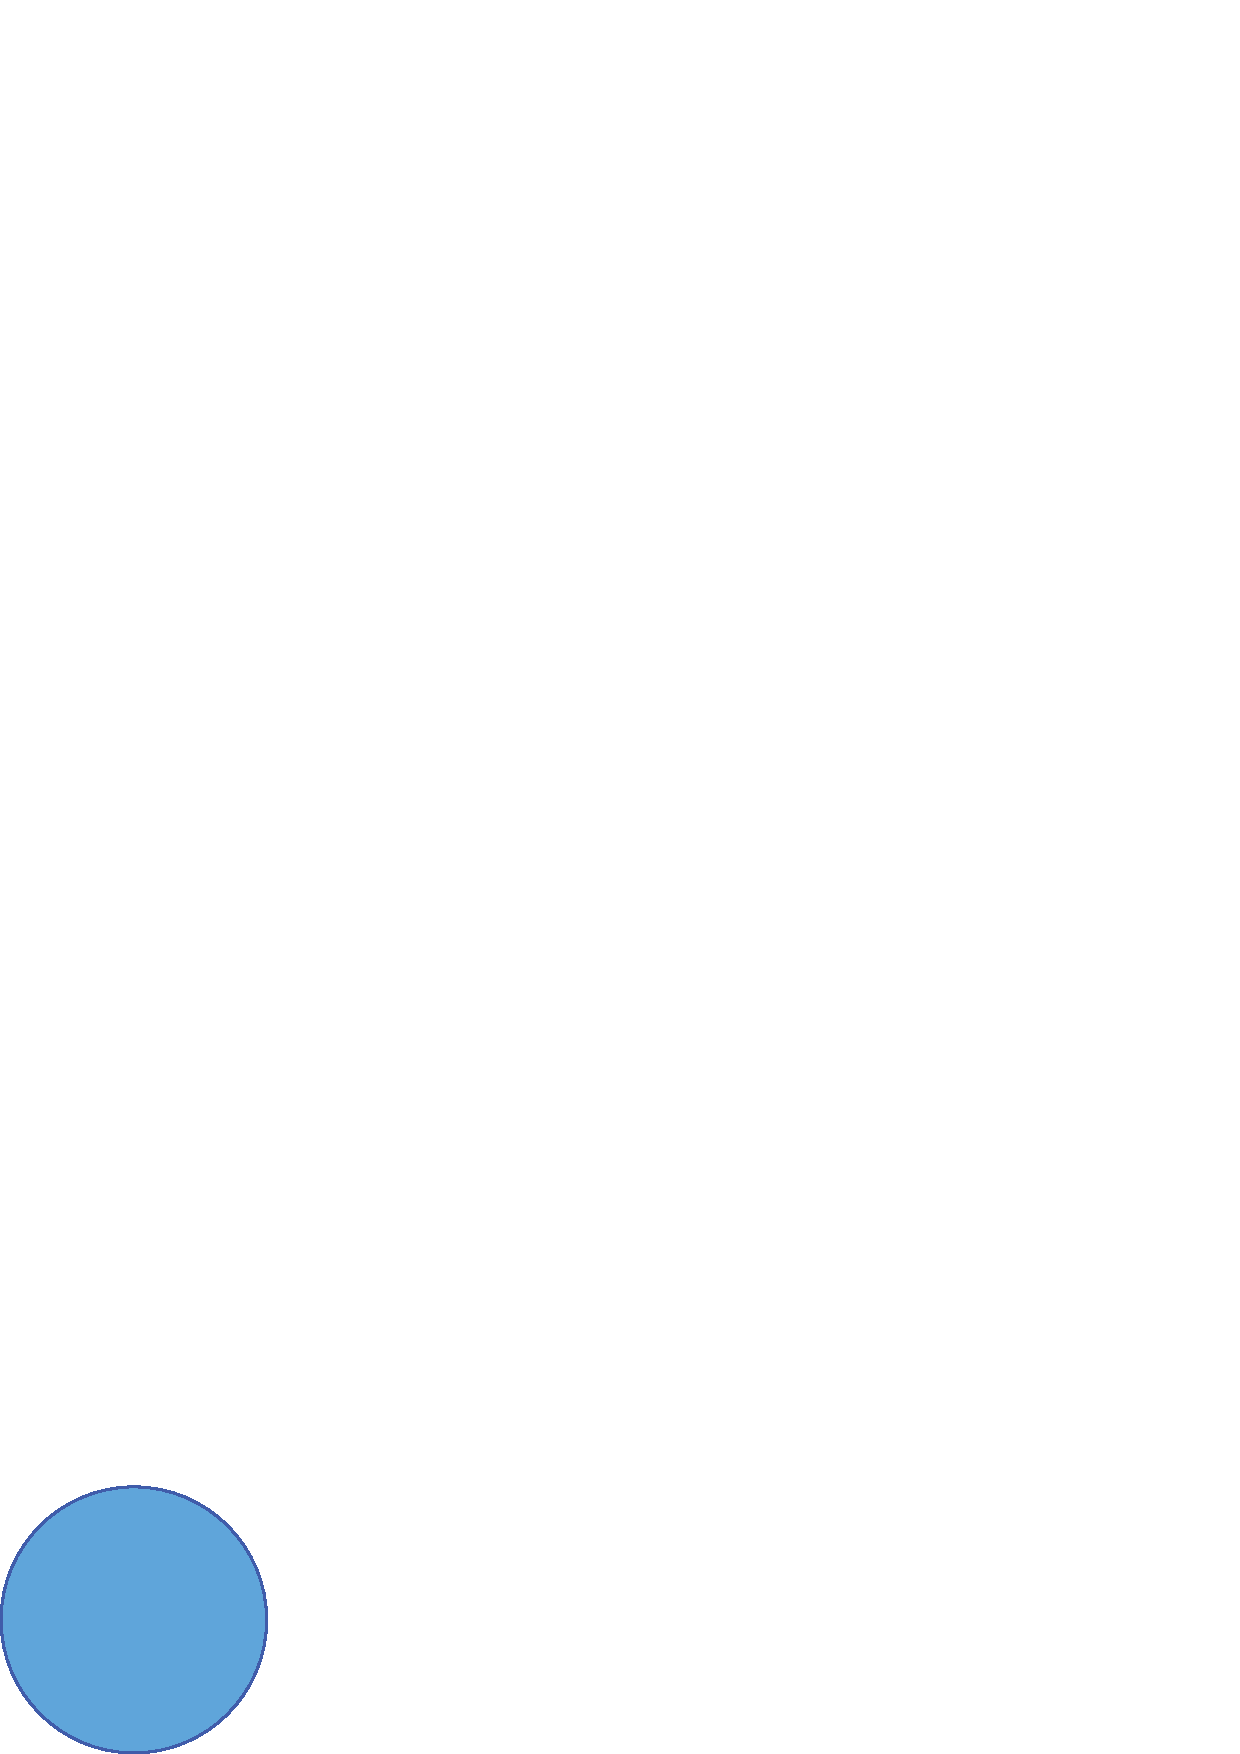
\includegraphics[width=40mm,bb=0 0 640 480]{image.jpg}}
    \end{center}
    \caption{図の例}
    \label{fig:sample1}
\end{figure}
\end{verbatim}
\end{itembox}

bbの指定は、上記のように{\tt *.tex} ファイルの中で指定してもいいが、
{\tt *.bb}ファイルを作っておく方法もある。
ターミナルで{\tt ebb}コマンドを使用すると{\tt *.bb}ファイルを簡単に作れる。


\begin{itembox}[l]{ebbコマンドの例}
\begin{verbatim}
% ebb image.jpg
\end{verbatim}
\end{itembox}


\verb|\includegraphics| を \verb|\fbox| に入れると、画像に枠を付けられる。

\verb|\caption| コマンドで図の見出しを指定できる。図の見出しは、図の下に表記するので注意。ここで指定した見出しが、図の目次に表示される。

\verb|\label| コマンドでは図の参照用ラベルを設定できる。本文中、\verb|\ref| コマンドで参照用ラベルを指定すると、対応した図の番号が自動的に挿入される。これも目次や参考文献と同様、最低二回のコンパイルが必要なので注意。

図を二つ横に並べたい場合は、次のように書く(図\ref{fig:sample2}、図\ref{fig:sample3})。

\begin{figure}[htbp]
  \begin{minipage}{0.5\hsize}
    \begin{center}
       \fbox{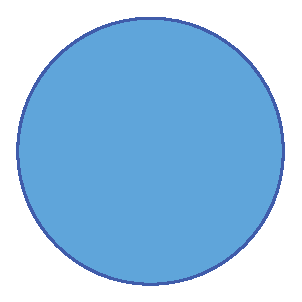
\includegraphics[width=40mm]{image.eps}}
    \end{center}
    \caption{図を並べる例1}
    \label{fig:sample2}
  \end{minipage}
  \begin{minipage}{0.5\hsize}
    \begin{center}
       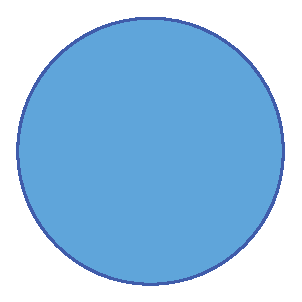
\includegraphics[width=40mm]{image.eps}
    \end{center}
    \caption{図を並べる例2、枠なし}
    \label{fig:sample3}
  \end{minipage}
\end{figure}

\begin{itembox}[l]{{\tt 03.tex}}
\begin{verbatim}
図を二つ横に並べたい場合は、次のように書く(図\ref{fig:sample2}、図\ref{fig:sample3})。

\begin{figure}[htbp]
  \begin{minipage}{0.5\hsize}
    \begin{center}
       \fbox{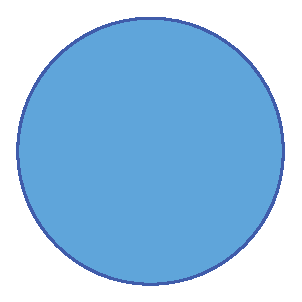
\includegraphics[width=40mm]{image.eps}}
    \end{center}
    \caption{図を並べる例1}
    \label{fig:sample2}
  \end{minipage}
  \begin{minipage}{0.5\hsize}
    \begin{center}
       \fbox{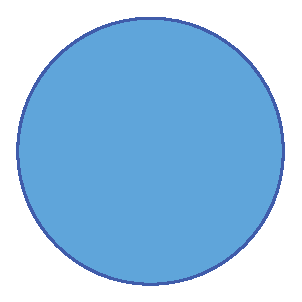
\includegraphics[width=40mm]{image.eps}}
    \end{center}
    \caption{図を並べる例2}
    \label{fig:sample3}
  \end{minipage}
\end{figure}
\end{verbatim}
\end{itembox}


\subsection{表}

表は次のように出力される(表\ref{tb:sample1})。

\begin{table}[htbp]
  \caption{表の例}
  \label{tb:sample1}
  \begin{center}
  \begin{tabular}{l|c|r}
    \hline
    種類	&味&評価\\\hline\hline
    ドラ焼き&甘い&好き\\\hline
    メロンパン&カリもふ&好き\\\hline
    クリームパン&神&すごく好き\\\hline
  \end{tabular}\end{center}
\end{table}

ソースでは次のようになっている。

\begin{itembox}[l]{{\tt 03.tex}}
\begin{verbatim}
表は次のように出力される(表\ref{tb:sample1})。

\begin{table}[htbp]
  \caption{表の例}
  \label{tb:sample1}
  \begin{center}
  \begin{tabular}{l|c|r}
    \hline
    種類	&味&評価\\\hline\hline
    ドラ焼き&甘い&好き\\\hline
    メロンパン&カリもふ&好き\\\hline
    クリームパン&神&すごく好き\\\hline
  \end{tabular}\end{center}
\end{table}
\end{verbatim}
\end{itembox}

{\tt htbp}や \verb|\caption| と \verb|\label| は図と同様。ただし表のタイトルは表の上に書く。

\verb|\begin{tabular}{l|{\tt \textbar}{\tt c}{\tt \textbar}\verb|r}|で横方向のセルを指定する。{\tt c}は中央揃え、{\tt l}は左揃え、{\tt r}は右揃えのセルを作る。{\tt \textbar}は垂直方向の罫線を表す。{\tt c}か{\tt l}か{\tt r}を必要なセルの数だけ並べて、セルの間に罫線が必要なら{\tt \textbar}を入れればよい。

セルの中の文字は、{\tt \&}で区切って並べる。行と行は \verb|\\| で区切る。水平方向の罫線が必要なら、\verb|\hline| を書く。

水平方向や垂直方向のセルの結合もできる。例を示すので、くわしくはぐぐろう。説明がめんどう。\verb|\multirow|、\verb|\multicolumn|、\verb|\cline| を使うとできる。

\begin{table}[htbp]
  \caption{セルを結合した例}
  \label{tb:sample2}
  \begin{center}
  \begin{tabular}{c|c|c}
    \hline
    ほげ&ふー&ばー\\\hline\hline
    \multirow{2}{*}{ほげほげ}&\multicolumn{2}{c}{ふーふー} \\\cline{2-3}
    &ふーふーふー&ばーばーばー\\\hline
  \end{tabular}
  \end{center}
\end{table}

\begin{itembox}[l]{{\tt 03.tex}}
\begin{verbatim}
\begin{table}[htbp]
  \caption{セルを結合した例}
  \label{tb:sample2}
  \begin{center}
  \begin{tabular}{c|c|c}
    \hline
    ほげ&ふー&ばー\\\hline\hline
    \multirow{2}{*}{ほげほげ}&\multicolumn{2}{c}{ふーふー} \\\cline{2-3}
    &ふーふーふー&ばーばーばー\\\hline
  \end{tabular}
  \end{center}
\end{table}
\end{verbatim}
\end{itembox}


\subsection{脚注}

脚注は \verb|\footnote| コマンドを使う。例えばこんな感じ\footnote{ページの下に小さく説明を出せる}。

\begin{itembox}[l]{{\tt 03.tex}}
\begin{verbatim}
例えばこんな感じ\footnote{ページの下に小さく説明を出せる}。
\end{verbatim}
\end{itembox}

\section{その他のコマンド}

ぐぐる\footnote{http://www.google.co.jp/}。

特殊なことは何もしていないテンプレートなので、ぐぐって出たことはだいたいそのまま何でも使える。

あるいは、このファイル自体も\LaTeX で書かれているわけだから、これの{\tt *.tex}を見るのもよいかもしれない。
  % 本文3
\chapter{結論}
\label{chap:conclusion}

この章では、結論らしいことをかく。

\section{まとめ}

\LaTeX の環境さえあればスタンダードな体裁の論文がたぶんだれでも作れる程度のテンプレートにはなっているはず。がんばって卒業しよう。


\section{大事なこと}

箇条書きで列挙する。

\begin{itemize}
 \item ぐぐる。これは単なる\LaTeX だし、\LaTeX はもう枯れた技術だから、調べれば文献はいくらでもある。
 \item 先生を頼る。
 \item 単位をきちんとる。
 \item 卒業する。
\end{itemize}


  % 本文4

\begin{acknowledgment}

このテンプレートを改造するにあたって、@kurokoboとインターネット上のいくつかの修士論文などを参考にしました。感謝いたします。

\end{acknowledgment}
  % 謝辞。要独自コマンド、include先参照のこと

\begin{bib}[100]

\bibliography{main}

\end{bib}
  % 参考文献。要独自コマンド、include先参照のこと
\appendix
\chapter{付録の例}

付録を無理矢理出力させるため、てきとうなことを書く。

\section{ほげ}

コマンドは本文と一緒。

\subsection{ふー}

本文と一緒。

\section{ほげほげ}

本文と一緒。

\subsection{ふーふー}

本文と一緒。
    % 付録

\end{document}
